\documentclass[journal]{IEEEtran}
%
% If IEEEtran.cls has not been installed into the LaTeX system files,
% manually specify the path to it like:
% \documentclass[journal]{../sty/IEEEtran}
\usepackage[T1]{fontenc}
\usepackage{cite}
\usepackage{amsmath,amssymb,amsfonts}
\usepackage{algorithmic}
\usepackage{graphicx}
\usepackage{textcomp}
\usepackage{xcolor}
\usepackage[section]{placeins}
\usepackage{mathrsfs}
\usepackage{subfigure}
\usepackage{physics}
\usepackage{tikz} 
\usepackage{scalefnt}
\usepackage{qcircuit}
\usepackage{tabularx} 
\usepackage{enumerate}
\usepackage{multirow}
\usepackage{caption}
\usepackage{hyperref} 

\usepackage[ruled,vlined]{algorithm2e}
\newcommand{\yx}[1]{{\color{magenta} [YX: #1]}}
\newcommand{\leaveout}[1]{}
\newtheorem{example}{Example}
\newcommand{\RNum}[1]{\uppercase\expandafter{\romannumeral #1\relax}}

% correct bad hyphenation here
\hyphenation{op-tical net-works semi-conduc-tor}


\begin{document}

\title{Quantum Circuit Transformation Based on Subgraph Isomorphism and Tabu Search}
%
%
% author names and IEEE memberships
% note positions of commas and nonbreaking spaces ( ~ ) LaTeX will not break
% a structure at a ~ so this keeps an author's name from being broken across
% two lines.
% use \thanks{} to gain access to the first footnote area
% a separate \thanks must be used for each paragraph as LaTeX2e's \thanks
% was not built to handle multiple paragraphs
%

\author{Michael~Shell,~\IEEEmembership{Member,~IEEE,}
        John~Doe,~\IEEEmembership{Fellow,~OSA,}
        and~Jane~Doe,~\IEEEmembership{Life~Fellow,~IEEE}% <-this % stops a space
\thanks{M. Shell was with the Department
of Electrical and Computer Engineering, Georgia Institute of Technology, Atlanta,
GA, 30332 USA e-mail: (see http://www.michaelshell.org/contact.html).}% <-this % stops a space
\thanks{J. Doe and J. Doe are with Anonymous University.}% <-this % stops a space
\thanks{Manuscript received April 19, 2005; revised August 26, 2015.}}


% The paper headers
\markboth{Journal of \LaTeX\ Class Files,~Vol.~14, No.~8, August~2015}%
{Shell \MakeLowercase{\textit{et al.}}: Bare Demo of IEEEtran.cls for IEEE Journals}
% The only time the second header will appear is for the odd numbered pages
% after the title page when using the twoside option.
% 
% *** Note that you probably will NOT want to include the author's ***
% *** name in the headers of peer review papers.                   ***
% You can use \ifCLASSOPTIONpeerreview for conditional compilation here if
% you desire.




% If you want to put a publisher's ID mark on the page you can do it like
% this:
%\IEEEpubid{0000--0000/00\$00.00~\copyright~2015 IEEE}
% Remember, if you use this you must call \IEEEpubidadjcol in the second
% column for its text to clear the IEEEpubid mark.



% use for special paper notices
%\IEEEspecialpapernotice{(Invited Paper)}




% make the title area
\maketitle

% As a general rule, do not put math, special symbols or citations
% in the abstract or keywords.
\begin{abstract}
The goal of quantum circuit transformation is to construct mappings from logical quantum circuits to physical ones in an acceptable amount of time, and in the meantime to introduce  as few auxiliary gates as possible. We present an effective approach to constructing the mappings. It consists of two keys steps: one makes use of a combined subgraph isomorphism and complement (CSIC) to initialize a mapping, the other dynamically adjusts the mapping by using a Tabu search based adjustment (TSA). Our experiments show that, compared with the wghtgraph recently considered in the literature, CSIC can save 22.26\% of auxiliary gates and reduce the depths of output circuits by 11.76\% on average in the initialization of the mapping, and  TSA has a better scalability than many state-of-the-art algorithms for adjusting mappings.
\end{abstract}

% Note that keywords are not normally used for peerreview papers.
\begin{IEEEkeywords}
Quantum circuit transformation  ,  Subgraph isomorphism , Initial mapping , Tabu search
\end{IEEEkeywords}

% For peer review papers, you can put extra information on the cover
% page as needed:
% \ifCLASSOPTIONpeerreview
% \begin{center} \bfseries EDICS Category: 3-BBND \end{center}
% \fi
%
% For peerreview papers, this IEEEtran command inserts a page break and
% creates the second title. It will be ignored for other modes.
\IEEEpeerreviewmaketitle
\section{Introduction}

The entanglement of a quantum system with its surrounding environment will lead to quantum decoherence. It is unrealistic to use quantum error correction in circuit mapping process, since there are only dozens of available qubits for quantum devices in the NISQ era~\cite{2018QuantumPreskill}. It is necessary to transform circuits by adding auxiliary gates to satisfy both logical and physical constraints, since quantum algorithms do not consider any hardware connectivity constraints. Hence, quantum circuit transformation is an important part of quantum circuit compilation. We need a set of highly efficient and automatic mapping procedures and adjustment routines to perform circuit transformation. In this process noise may be introduced, which brings a huge challenge to circuit compilation because noise has a significant impact on the final circuit and may make the result meaningless. 

In the current work, we adjust the lifetime of qubits through parallelization, and use SubgraphMatching~\cite{Sun2020} to generate partial isomorphic subgraphs of logical circuits %$LC$
and physical circuits %$PC$
as part of the initial mapping. The advantage of the initial mapping result is that we use the appropriate subgraph isomorphism and the two-way connection of the logical circuit and the physical circuit to obtain a dense initial mapping, which avoids certain nodes from being mapped to remote locations. We use Tabu search~\cite{Glover1990} to generate circuits that can be executed on physical devices. Tabu search can avoid falling into local optimum and swapping the recently swapped qubits, thereby improve the parallelism of quantum gates. We add SWAP gates associated with the gates on the shortest path to the candidate set, which greatly reduces the search space and improves the search speed. Our heuristic function not only considers the current gates but also the constraints of the gates already considered.

We compare CSIC with the state-of-the-art initial mapping methods wghtgraph~\cite{2020Qubit} and optm~\cite{Zulehner2017}. On average, the auxiliary gates of the CSIC algorithm are reduced by 22.44\% (resp. 27.02\%), and the depths are reduced by 11.25\% (resp. 14.12\%). We compare TSA with wgtgraph~\cite{2020Qubit} and SABRE~\cite{Li2018}. On the one hand, TSA can handle 159 circuits in a few minutes, while the  other two adjustment algorithms are difficult to handle medium-sized or large circuits. On the other hand, the number of SWAP gates added by wgtgraph is 26.87\% (resp. 24.89\%) smaller than that of  TSA on average. Among the 159 circuits that we also test with SABRE, only 29  can be successfully mapped within the five-minute limit.

%, but needs to control the decisiveness of the behind gates in the heuristic function.
The main contributions of this paper are as follows.
	\begin{enumerate}
	\item We propose to use the combined subgraph isomorphism algorithm to generate part of the initial mapping
          %, which can be reduced to subgraph isomorphism. Thus we use a suitable subgraph isomorphism algorithm to generate part of the initial mapping
    and then complete the mapping based on the connectivity between qubits.
	\item We present a heuristic circuit adjustment algorithm based on Tabu search~\cite{Glover1990}, which can handle large circuits in a shorter time at a lower cost, compared with existing precise search and heuristic algorithms.
          %, it can complete the circuit transformation in a shorter time. 
	\item  We put forward a look-ahead heuristic function that considers both the current gates and the  gates yet to be processed. It filters out SWAP gates that are beneficial to the current gates and also bring closer the gates to be processed.
	\item We test 159 circuits, and the results show that the initial mapping generated by our method requires to insert fewer SWAP gates, and the adjustment algorithm can be extended to handle medium-sized and large circuits.
	\end{enumerate}

The rest of this paper is organized as follows.
In Section~\ref{Related work} we discuss some related work. 
In Section~\ref{Background} we recall some background of quantum computing and quantum information. In Section~\ref{Problem Description and Solution Outline}
we introduce the problem of  quantum circuit transformation provide our solution by describing our algorithm in detail.
The experimental results are reported in Section~\ref{Experiment}. 
The last section concludes the paper and discusses some future research.


\section{Related work}
\label{Related work}
Quantum technology has been applied in practice, but large quantum computers have not yet been built. Most of the contributions of quantum information to computer science are still in the theoretical stage. In 2017, IBM developed the first 5-qubit backend called IBM QX2, followed by the 16-qubit backend  IBM QX3. The revised versions of them are called IBM QX4 and IBM QX5, respectively. IBM Q Experience \cite{ibm} provides the public with free quantum computer resources on the cloud and opens source the quantum computing software framework Qiskit \cite{qiskit}. 

Users of these early quantum computers mainly rely on quantum circuits to implement quantum algorithms. They design logical circuits which then go through the step of circuit transformation in order to map logical qubits to physical ones before the logical circuits are executed in physical devices. A big challenge for quantum information is the problem of quantum decoherence. Due to the decoherence of qubits, quantum gates need to be applied in a coherent period as the time for a qubit to stay in a coherent state is very short. The longest coherence time of a superconducting quantum chip is still within 10us-100us. 

There are several initial mapping methods. Paler~\cite{Paler2018} has showed that the initial mapping has an important influence on quantum circuit transformation. He proposed a heuristic method to find the initial mapping. Just by placing qubits in different positions from the default trivial placement
 in the actual circuit instances on the actual NISQ device, the time cost can be reduced by up to 10\%. Li et al.~\cite{Li2018} have proposed a novel reverse traversal technique, which determines the initial mapping by considering the entire circuit. Zhou et al.~\cite{Xiangzhen2020} have put forward an annealing algorithm to find an initial mapping, but it is unstable. In \cite{2020Qubit}, Li et al. have considered the subgraph isomorphism algorithm wghtgraph to generate an initial mapping, which is the most recent result, so we will compare with it.

The goal of circuit adjustment algorithm is to minimize the number of auxiliary SWAP gates. There are currently five main methods for solving the quantum circuit adjustment problem.
\begin{itemize}
  \item
\emph{Unitary matrix decomposition algorithm.} It is used in \cite{2019CNOT,2019Quantum} to rearrange the quantum circuit from the beginning while retaining the input circuit. It can be applied to a broad class of circuits consisting of generic gate sets, but the results are not as efficient as a compiler designed specifically for this task.
\item
\emph{Converting into some existing problems.} This approach converts the quantum circuit transformation problem into some existing problems, such as AI planning~\cite{2017Temporal,2018Integer}, Integer Linear Programming (ILP)~\cite{2019Almeida}, or Satisfiability Modulo Theories (SMT)~\cite{2019Murali}. Existing tools for those problems are then used to find acceptable results. The approach cannot take advantage of certain properties of quantum mapping, which is a drawback. Furthermore, as the time cost is usually long, it can only handle small quantum circuits.
\item
\emph{Exact methods.}
Siraichi et al.~\cite{2018QubitSiraichi} have proposed an exact method. It will iterate all possible mappings for all dependencies, so it is only suitable for simple quantum architecture and cannot be extended to complex quantum architectures.
\item
\emph{Graph theory.} 
In~\cite{Shafaei2013}, Shafaei et al. have used the minimum linear permutation solution in graph theory to model the problem of reducing the interaction distance. The idea is to first divide a given circuit into several subcircuits and apply the minimum linear permutation solution, respectively. Then we turn non-adjacent gates in the subcircuits into adjacent gates by adding auxiliary gates. Finally, we can use the minimum linear permutation solution to find an appropriate permutation and use bubble sort to calculate the number of necessary SWAP gates. In \cite{Guerreschi2018,Matsuo2019}, a two-step method is used to reduce the quantum circuit transformation to the graph problem to minimize the number of auxiliary gates, based on the graph coloring problem and the largest subgraph isomorphism problem.
\item
\emph{Heuristic search.}
Heuristic search uses an evaluation function to obtain an acceptable solution in exponential time. Zulehner et al. \cite{Zulehner2017} have suggested to layer the circuits, then determine compatible mappings for each of these layers to add as few auxiliary gates as possible. Zhou et al.~\cite{Xiangzhen2020} have designed a heuristic search algorithm with a novel selection mechanism. Instead of choosing the operation with the lowest cost to apply, one can look forward one step and then choose the best continuous operation. In this way, the algorithm can effectively avoid local minimum. Moreover, a pruning mechanism is introduced to reduce the search space's size and ensure that the program terminates in a reasonable amount of time.
%The overall time complexity of this algorithm is $O(|V|^{4})$, where $V$ is.

Li et al.~\cite{Li2018} have proposed a SWAP-based search algorithm SABRE. Compared with previous search algorithms based on exhaustive mapping, SABRE
%achieves exponential search complexity and ensures the scalability of SABRE to
can adapt to large quantum circuits in the NISQ era. In \cite{Cowtan2019}, a routing algorithm called $t\ket{ket}$  ensures that any quantum circuit can be compiled into any architecture. The algorithm is divided into four stages: decomposing the input circuit into time steps, determining the initial mapping, routing across time steps, and finally cleaning up. The heuristics in $t\ket{ket}$ give the same or better results than other circuit transformation systems in terms of the depth and the total number of gates in the compiled circuit, with much shorter running time, and can handle larger circuits. In \cite{Tannu2019},  a variation-aware qubit movement strategy is proposed. It takes advantage of the change in error rate and a change-aware quantum circuit transformation strategy by trying to select the route with the lowest probability of failure. This strategy uses the error rate of  SWAPs to allocate logical qubits to physical qubits, thus avoiding paths with high error rates as much as possible.
\end{itemize}

Among the existing methods above, wghtgraph~\cite{2020Qubit} and optm~\cite{Zulehner2017} are probably the most effective initial mapping ones. As to circuit adjustment algorithms, wgtgraph~\cite{2020Qubit} and SABRE~\cite{Li2018} represent the state of the art. Therefore, we choose to compare our solution with them in Section~\ref{Experiment}.


\section{Preliminary}
\label{Background}
In this section we introduce some notions and notations of quantum computing and quantum information.
\begin{figure*}[htbp]
	{
  \scalefont{0.8}
  \qquad\,
	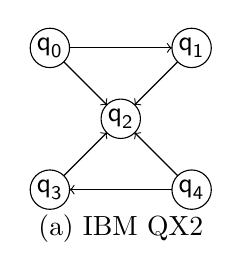
\begin{tikzpicture}
	% \draw[help Lines] (0,0) grid (11,3);
		% IBM QX2
	\node at (1.8,0.4){(a) IBM QX2};
	% label
	\node at (0.9,2.7){$\textsf{q}_\textsf{0}$};
	\draw [black, thin] (0.9,2.7) circle [radius=0.25];
	\node at (2.7,2.7){$\textsf{q}_\textsf{1}$};
	\draw [black, thin] (2.7,2.7) circle [radius=0.25];
	\node at (1.8,1.8){$\textsf{q}_\textsf{2}$};
	\draw [black, thin] (1.8,1.8)circle [radius=0.25];
	\node at (0.9,0.9){$\textsf{q}_\textsf{3}$};
	\draw [black, thin] (0.9,0.9) circle [radius=0.25];
	\node at (2.7,0.9){$\textsf{q}_\textsf{4}$};
	\draw [black, thin] (2.7,0.9) circle [radius=0.25];
	% -
	\draw [->,thin] (1.15,2.7) -- (2.45,2.7);
	
	\draw [<-,thin] (1.15,0.9) -- (2.45,0.9);

	%x
	\draw [->,thin] (1.075,2.525) -- (1.625,1.975);
	\draw [->,thin] (2.525,2.525) -- (1.975,1.975);
	\draw [->,thin] (1.075,1.075) -- (1.625,1.625);
	\draw [->,thin] (2.525,1.075) -- (1.975,1.625);
  \end{tikzpicture}
  \quad
  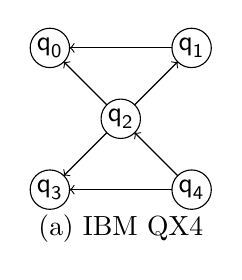
\begin{tikzpicture}
    % \draw[help Lines] (0,0) grid (11,3);
      % IBM QX2
    \node at (1.8,0.4){(a) IBM QX4};
    % label
    \node at (0.9,2.7){$\textsf{q}_\textsf{0}$};
    \draw [black, thin] (0.9,2.7) circle [radius=0.25];
    \node at (2.7,2.7){$\textsf{q}_\textsf{1}$};
    \draw [black, thin] (2.7,2.7) circle [radius=0.25];
    \node at (1.8,1.8){$\textsf{q}_\textsf{2}$};
    \draw [black, thin] (1.8,1.8)circle [radius=0.25];
    \node at (0.9,0.9){$\textsf{q}_\textsf{3}$};
    \draw [black, thin] (0.9,0.9) circle [radius=0.25];
    \node at (2.7,0.9){$\textsf{q}_\textsf{4}$};
    \draw [black, thin] (2.7,0.9) circle [radius=0.25];
  
    
    % -
    \draw [<-,thin] (1.15,2.7) -- (2.45,2.7);
    
    \draw [<-,thin] (1.15,0.9) -- (2.45,0.9);
  
    %x
    \draw [<-,thin] (1.075,2.525) -- (1.625,1.975);
    \draw [<-,thin] (2.525,2.525) -- (1.975,1.975);
    \draw [<-,thin] (1.075,1.075) -- (1.625,1.625);
    \draw [->,thin] (2.525,1.075) -- (1.975,1.625);
    \end{tikzpicture}
  \quad
  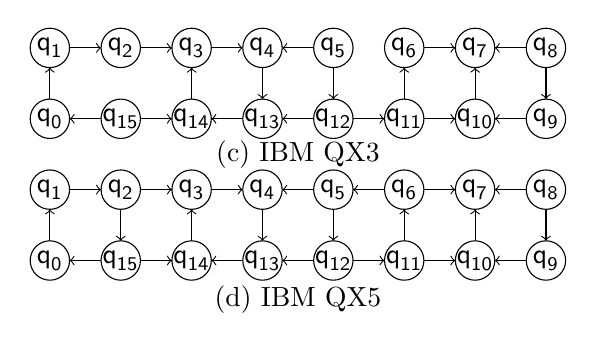
\begin{tikzpicture}
			
    \node at (3.15,0){(d) IBM QX5};
    \node at (3.15,1.85){(c) IBM QX3};
      %QX5
      %-
    \draw [black, thin] (0,2.3) circle [radius=0.25];
    \draw [<-,thin] (0.25,2.3) -- (0.65,2.3);
    \draw [black, thin] (0.9,2.3) circle [radius=0.25];
    \draw [->,thin] (1.15,2.3) -- (1.55,2.3);
    \draw [black, thin] (1.8,2.3) circle [radius=0.25];
    \draw [<-,thin] (2.05,2.3) -- (2.45,2.3);
    \draw [black, thin] (2.7,2.3) circle [radius=0.25];
    \draw [<-,thin] (2.95,2.3) -- (3.35,2.3);
    \draw [black, thin] (3.6,2.3) circle [radius=0.25];
    \draw [->,thin] (3.85,2.3) -- (4.25,2.3);
    \draw [black, thin] (4.5,2.3) circle [radius=0.25];
    \draw [->,thin] (4.75,2.3) -- (5.15,2.3);
    \draw [black, thin] (5.4,2.3) circle [radius=0.25];
    \draw [<-,thin] (5.65,2.3) -- (6.05,2.3);
    \draw [black, thin] (6.3,2.3) circle [radius=0.25];
  
    % |
    \draw [->,thin] (0,2.55) -- (0,2.95);
    \draw [->,thin] (1.8,2.55) -- (1.8,2.95);
    \draw [<-,thin] (2.7,2.55) -- (2.7,2.95);
    \draw [<-,thin] (3.6,2.55) -- (3.6,2.95);
    \draw [->,thin] (4.5,2.55) -- (4.5,2.95);
    \draw [->,thin] (5.4,2.55) -- (5.4,2.95);
    \draw [<-,thin] (6.3,2.55) -- (6.3,2.95);
    %-
  \draw [black, thin] (0,3.2) circle [radius=0.25];
  \draw [->,thin] (0.25,3.2) -- (0.65,3.2);
  \draw [black, thin] (0.9,3.2) circle [radius=0.25];
  \draw [->,thin] (1.15,3.2) -- (1.55,3.2);
  \draw [black, thin] (1.8,3.2) circle [radius=0.25];
  \draw [->,thin] (2.05,3.2) -- (2.45,3.2);
  \draw [black, thin] (2.7,3.2) circle [radius=0.25];
  \draw [<-,thin] (2.95,3.2) -- (3.35,3.2);
  \draw [black, thin] (3.6,3.2) circle [radius=0.25];
  
  \draw [black, thin] (4.5,3.2) circle [radius=0.25];
  \draw [->,thin] (4.75,3.2) -- (5.15,3.2);
  \draw [black, thin] (5.4,3.2) circle [radius=0.25];
  \draw [<-,thin] (5.65,3.2) -- (6.05,3.2);
  \draw [black, thin] (6.3,3.2) circle [radius=0.25];
    
    % label
    \node at (0,0.5){$\textsf{q}_\textsf{0}$};
    \node at (0.9,0.5){$\textsf{q}_\textsf{15}$};
    \node at (1.8,0.5){$\textsf{q}_\textsf{14}$};
    \node at (2.7,0.5){$\textsf{q}_\textsf{13}$};
    \node at (3.6,0.5){$\textsf{q}_\textsf{12}$};
    \node at (4.5,0.5){$\textsf{q}_\textsf{11}$};
    \node at (5.4,0.5){$\textsf{q}_\textsf{10}$};
    \node at (6.3,0.5){$\textsf{q}_\textsf{9}$};
  
    \node at (0,1.4){$\textsf{q}_\textsf{1}$};
    \node at (0.9,1.4){$\textsf{q}_\textsf{2}$};
    \node at (1.8,1.4){$\textsf{q}_\textsf{3}$};
    \node at (2.7,1.4){$\textsf{q}_\textsf{4}$};
    \node at (3.6,1.4){$\textsf{q}_\textsf{5}$};
    \node at (4.5,1.4){$\textsf{q}_\textsf{6}$};
    \node at (5.4,1.4){$\textsf{q}_\textsf{7}$};
    \node at (6.3,1.4){$\textsf{q}_\textsf{8}$};
  
      %QX5
      %-
      \draw [black, thin] (0,0.5) circle [radius=0.25];
      \draw [<-,thin] (0.25,0.5) -- (0.65,0.5);
      \draw [black, thin] (0.9,0.5) circle [radius=0.25];
      \draw [->,thin] (1.15,0.5) -- (1.55,0.5);
      \draw [black, thin] (1.8,0.5) circle [radius=0.25];
      \draw [<-,thin] (2.05,0.5) -- (2.45,0.5);
      \draw [black, thin] (2.7,0.5) circle [radius=0.25];
      \draw [<-,thin] (2.95,0.5) -- (3.35,0.5);
      \draw [black, thin] (3.6,0.5) circle [radius=0.25];
      \draw [->,thin] (3.85,0.5) -- (4.25,0.5);
      \draw [black, thin] (4.5,0.5) circle [radius=0.25];
      \draw [->,thin] (4.75,0.5) -- (5.15,0.5);
      \draw [black, thin] (5.4,0.5) circle [radius=0.25];
      \draw [<-,thin] (5.65,0.5) -- (6.05,0.5);
      \draw [black, thin] (6.3,0.5) circle [radius=0.25];
    
      % |
      \draw [->,thin] (0,0.75) -- (0,1.15);
      \draw [<-,thin] (0.9,0.75) -- (0.9,1.15);
      \draw [->,thin] (1.8,0.75) -- (1.8,1.15);
      \draw [<-,thin] (2.7,0.75) -- (2.7,1.15);
      \draw [<-,thin] (3.6,0.75) -- (3.6,1.15);
      \draw [->,thin] (4.5,0.75) -- (4.5,1.15);
      \draw [->,thin] (5.4,0.75) -- (5.4,1.15);
      \draw [<-,thin] (6.3,0.75) -- (6.3,1.15);
      %-
    \draw [black, thin] (0,1.4) circle [radius=0.25];
    \draw [->,thin] (0.25,1.4) -- (0.65,1.4);
    \draw [black, thin] (0.9,1.4) circle [radius=0.25];
    \draw [->,thin] (1.15,1.4) -- (1.55,1.4);
    \draw [black, thin] (1.8,1.4) circle [radius=0.25];
    \draw [->,thin] (2.05,1.4) -- (2.45,1.4);
    \draw [black, thin] (2.7,1.4) circle [radius=0.25];
    \draw [<-,thin] (2.95,1.4) -- (3.35,1.4);
    \draw [black, thin] (3.6,1.4) circle [radius=0.25];
    \draw [<-,thin] (3.85,1.4) -- (4.25,1.4);
    \draw [black, thin] (4.5,1.4) circle [radius=0.25];
    \draw [->,thin] (4.75,1.4) -- (5.15,1.4);
    \draw [black, thin] (5.4,1.4) circle [radius=0.25];
    \draw [<-,thin] (5.65,1.4) -- (6.05,1.4);
    \draw [black, thin] (6.3,1.4) circle [radius=0.25];
      
      % label
      \node at (0,2.3){$\textsf{q}_\textsf{0}$};
      \node at (0.9,2.3){$\textsf{q}_\textsf{15}$};
      \node at (1.8,2.3){$\textsf{q}_\textsf{14}$};
      \node at (2.7,2.3){$\textsf{q}_\textsf{13}$};
      \node at (3.6,2.3){$\textsf{q}_\textsf{12}$};
      \node at (4.5,2.3){$\textsf{q}_\textsf{11}$};
      \node at (5.4,2.3){$\textsf{q}_\textsf{10}$};
      \node at (6.3,2.3){$\textsf{q}_\textsf{9}$};
    
      \node at (0,3.2){$\textsf{q}_\textsf{1}$};
      \node at (0.9,3.2){$\textsf{q}_\textsf{2}$};
      \node at (1.8,3.2){$\textsf{q}_\textsf{3}$};
      \node at (2.7,3.2){$\textsf{q}_\textsf{4}$};
      \node at (3.6,3.2){$\textsf{q}_\textsf{5}$};
      \node at (4.5,3.2){$\textsf{q}_\textsf{6}$};
      \node at (5.4,3.2){$\textsf{q}_\textsf{7}$};
      \node at (6.3,3.2){$\textsf{q}_\textsf{8}$};
    \end{tikzpicture}
  \quad
  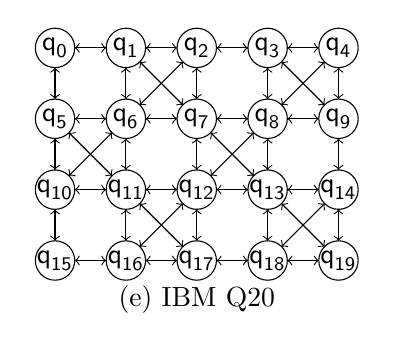
\begin{tikzpicture}
    
      % IBM Q20
      \node at (1.8,0){(e) IBM Q20};
    % Q20
    \draw [black, thin] (0,0.5) circle [radius=0.25];
    \draw [<->,thin] (0.25,0.5) -- (0.65,0.5);
    \draw [black, thin] (0.9,0.5) circle [radius=0.25];
    \draw [<->,thin] (1.15,0.5) -- (1.55,0.5);
    \draw [black, thin] (1.8,0.5) circle [radius=0.25];
    \draw [<->,thin] (2.05,0.5) -- (2.45,0.5);
    \draw [black, thin] (2.7,0.5) circle [radius=0.25];
    \draw [<->,thin] (2.95,0.5) -- (3.35,0.5);
    \draw [black, thin] (3.6,0.5) circle [radius=0.25];
  
    \node at (0,0.5) {$\textsf{q}_\textsf{15}$};
    \node at (0.9,0.5){$\textsf{q}_\textsf{16}$};
    \node at (1.8,0.5){$\textsf{q}_\textsf{17}$};
    \node at (2.7,0.5){$\textsf{q}_\textsf{18}$};
    \node at (3.6,0.5){$\textsf{q}_\textsf{19}$};
    % |
    \draw [<->,thin] (0,0.75) -- (0,1.15);
    \draw [<->,thin] (0.9,0.75) -- (0.9,1.15);
    \draw [<->,thin] (1.8,0.75) -- (1.8,1.15);
    \draw [<->,thin] (2.7,0.75) -- (2.7,1.15);
    \draw [<->,thin] (3.6,0.75) -- (3.6,1.15);
  
    \draw [black, thin] (0,1.4) circle [radius=0.25];
    \draw [<->,thin] (0.25,1.4) -- (0.65,1.4);
    \draw [black, thin] (0.9,1.4) circle [radius=0.25];
    \draw [<->,thin] (1.15,1.4) -- (1.55,1.4);
    \draw [black, thin] (1.8,1.4)circle [radius=0.25];
    \draw [<->,thin] (2.05,1.4) -- (2.45,1.4);
    \draw [black, thin] (2.7,1.4) circle [radius=0.25];
    \draw [<->,thin] (2.95,1.4) -- (3.35,1.4);
    \draw [black, thin] (3.6,1.4) circle [radius=0.25];
    % label
    \node at (0,1.4) {$\textsf{q}_\textsf{10}$};
    \node at (0.9,1.4){$\textsf{q}_\textsf{11}$};
    \node at (1.8,1.4){$\textsf{q}_\textsf{12}$};
    \node at (2.7,1.4){$\textsf{q}_\textsf{13}$};
    \node at (3.6,1.4){$\textsf{q}_\textsf{14}$};
    % |
    \draw [<->,thin] (0,1.65) -- (0,2.05);
    \draw [<->,thin] (0.9,1.65)-- (0.9,2.05);
    \draw [<->,thin] (1.8,1.65) -- (1.8,2.05);
    \draw [<->,thin] (2.7,1.65) -- (2.7,2.05);
    \draw [<->,thin] (3.6,1.65) -- (3.6,2.05);
  
    \draw [black, thin] (0,2.3) circle [radius=0.25];
    \draw [<->,thin] (0.25,2.3) -- (0.65,2.3);
    \draw [black, thin] (0.9,2.3) circle [radius=0.25];
    \draw [<->,thin] (1.15,2.3) -- (1.55,2.3);
    \draw [black, thin] (1.8,2.3)circle [radius=0.25];
    \draw [<->,thin] (2.05,2.3) -- (2.45,2.3);
    \draw [black, thin] (2.7,2.3) circle [radius=0.25];
    \draw [<->,thin] (2.95,2.3) -- (3.35,2.3);
    \draw [black, thin] (3.6,2.3) circle [radius=0.25];
    % label
    \node at (0,2.3) {$\textsf{q}_\textsf{5}$};
    \node at (0.9,2.3){$\textsf{q}_\textsf{6}$};
    \node at (1.8,2.3){$\textsf{q}_\textsf{7}$};
    \node at (2.7,2.3){$\textsf{q}_\textsf{8}$};
    \node at (3.6,2.3){$\textsf{q}_\textsf{9}$};
    % |
    \draw [<->,thin] (0,2.55) -- (0,2.95);
    \draw [<->,thin] (0.9,2.55)-- (0.9,2.95);
    \draw [<->,thin] (1.8,2.55) -- (1.8,2.95);
    \draw [<->,thin] (2.7,2.55) -- (2.7,2.95);
    \draw [<->,thin] (3.6,2.55) -- (3.6,2.95);
  
    \draw [black, thin] (0,3.2) circle [radius=0.25];
    \draw [<->,thin] (0.25,3.2) -- (0.65,3.2);
    \draw [black, thin] (0.9,3.2) circle [radius=0.25];
    \draw [<->,thin] (1.15,3.2) -- (1.55,3.2);
    \draw [black, thin] (1.8,3.2)circle [radius=0.25];
    \draw [<->,thin] (2.05,3.2) -- (2.45,3.2);
    \draw [black, thin] (2.7,3.2) circle [radius=0.25];
    \draw [<->,thin] (2.95,3.2) -- (3.35,3.2);
    \draw [black, thin] (3.6,3.2) circle [radius=0.25];
    % label
    \node at (0,3.2) {$\textsf{q}_\textsf{0}$};
    \node at (0.9,3.2){$\textsf{q}_\textsf{1}$};
    \node at (1.8,3.2){$\textsf{q}_\textsf{2}$};
    \node at (2.7,3.2){$\textsf{q}_\textsf{3}$};
    \node at (3.6,3.2){$\textsf{q}_\textsf{4}$};
  
    %x
    \draw [<->,thin] (1.075,0.675) -- (1.625,1.225);
    \draw [<->,thin] (1.075,1.225) -- (1.625,0.675);
    \draw [<->,thin] (2.875,0.675) -- (3.425,1.225);
    \draw [<->,thin] (2.875,1.225) -- (3.425,0.675);
      %3
    \draw [<->,thin] (1.075,2.475) -- (1.625,3.025);
    \draw [<->,thin] (1.075,3.025) -- (1.625,2.475);
    \draw [<->,thin] (2.875,2.475) -- (3.425,3.025);
    \draw [<->,thin] (2.875,3.025) -- (3.425,2.475);
      % 2
    \draw [<->,thin] (0.175,2.125) -- (0.725,1.575);
    \draw [<->,thin] (0.175,1.575) -- (0.725,2.125);
    \draw [<->,thin] (1.975,2.125) -- (2.525,1.575);
    \draw [<->,thin] (1.975,1.575) -- (2.525,2.125);
    \end{tikzpicture}
}


\caption{IBM QX architectures}
\label{IBM}
\end{figure*}
%\paragraph{Qubits}
Classical information is stored in bits, while quantum information is stored in qubits. 
Besides two basic states $\ket{0}$ and $\ket{1}$,
a qubit can be in any linear superposition state like $\ket{\phi}=a\ket{0}+b\ket{1}$,
where $a,b\in \mathbb{C}$ satisfy the condition $|a|^{2}+|b|^{2}=1$.
The intuition is that $\ket{\phi}$ is in the state $\ket{0}$ with the probability $|a|^{2}$ or in the state $\ket{1}$ with the probability $|b|^{2}$.
We use letters $\textsf{q}$ and $\textit{q}$ in different fonts to represent physical qubits and logical qubits.

%\paragraph{Quantum Gates}
By applying quantum gates to qubits, we can change their states.
For example, the Hadamard gate (H gate) can be applied on a single qubit, while the CNOT gate can be applied on two qubits. Their representations in terms of  gate symbols and their semantics in terms of matrices are shown in Fig.~\ref{common_gates}. 
{
\begin{figure}[htbp]
	 \scalefont{1.0}
	 \begin{center}
	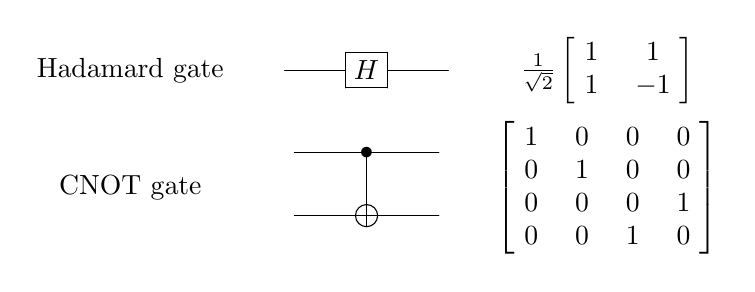
\begin{tikzpicture}
	% CNOT
	\node at (7,0){	CNOT gate };
	\node at (10,0){	
		\Qcircuit @C=2.2em @R=1.75em {
		 & \ctrl{1}  & \qw 	 \\
		 &\targ  	 & \qw   \\	    			}};
	\node at (13,0){\vspace{10em}
				$\begin{bmatrix}
					\ 1\ & 0\ & 0\ & 0\ \\
					\ 0\ & 1\ & 0\ & 0\ \\
					\ 0\ & 0\ & 0\ & 1\ \\
					\ 0\ & 0\ & 1\ & 0\ 
				\end{bmatrix}$
	};

		% T
% \node at (7,1.1){	$\frac{\pi}{8}$ gate };
% \node at (10,1.1){	\Qcircuit @C=2.2em @R=1.75em {
% 	 & \gate{T}  & \qw 	 \\						 
% }};
% \node at (13,1.1){\vspace{10em}
% 			$\begin{bmatrix}
% 				\ 1\ & 0\  \\
% 				\ 0\ & e^{i\pi/4}\ \\
% 			\end{bmatrix}$
% };
% phase gate
% \node at (7,2.2){	phase gate };
% \node at (10,2.2){	
% 	\Qcircuit @C=2.2em @R=1.75em {
% 	 & \gate{S}  & \qw 	 \\						 
% }};
% \node at (13,2.2){\vspace{10em}
% 			$\begin{bmatrix}
% 				\ 1\ & 0\  \\
% 				\ 0\ & i\ \\
% 			\end{bmatrix}$
% };

% Z gate
%\node at (7,3.3){	Pauli-Z gate };
%\node at (10,3.3){	
%	\Qcircuit @C=2.2em @R=1.75em {
%	 & \gate{Z}  & \qw 	 \\						 
%}};
%\node at (13,3.3){\vspace{10em}
%			$\begin{bmatrix}
%				\ 1\ & 0\  \\
%				\ 0\ & -1\ \\
%			\end{bmatrix}$
%};

% Y gate
%\node at (7,4.4){	Pauli-Y gate };
%\node at (10,4.4){	
%	\Qcircuit @C=2.2em @R=1.75em {
%	 & \gate{Y}  & \qw 	 \\						 
%}};
%\node at (13,4.4){\vspace{10em}
%			$\begin{bmatrix}
%				\ 1\ & -i\  \\
%				\ i\ & 0\ \\
%			\end{bmatrix}$
%};
% X gate
%\node at (7,5.5){	Pauli-X gate };
%\node at (10,5.5){	
%	\Qcircuit @C=2.2em @R=1.75em {
%	 & \gate{X}  & \qw 	 \\						 
%}};
%\node at (13,5.5){\vspace{10em}
%			$\begin{bmatrix}
%				\ 0\ & 1\  \\
%				\ 1\ & 0\ \\
%			\end{bmatrix}$
%};
% H
	% IBM Q20
	\node at (7,1.5){	Hadamard gate };
	\node at (10,1.5){	\Qcircuit @C=2.2em @R=1.75em {
		 & \gate{H}  & \qw 	 \\  						 
	}};
	\node at (13,1.5){\vspace{10em}
				$\frac{1}{\sqrt{2}}\begin{bmatrix}
					\ 1\ & 1\ \\
					\ 1\ & -1\ 
				\end{bmatrix}$
	};
\end{tikzpicture}
\end{center}
\caption{The symbols of two quantum gates and their matrices}\label{common_gates}
\end{figure}	 

}

%\paragraph{Quantum Circuit}
A quantum logical circuit 
consists of quantum gates interconnected by quantum wires~\cite{Daei2020}; see Fig.~\ref{OriginalCircuit} for an example.
A quantum wire is a mechanism for moving quantum data from one location to another.
Each line represents a qubit, and the gates on the lines act on the corresponding qubits.
The execution order of a quantum logical circuit  is from left to right.
The width %$w$ 
of a circuit refers to the number of qubits in the circuit.
The depth %$d$ 
of a circuit refers to the number of layers executing in parallel.
For example, the depth of the circuit in Fig.~\ref{OriginalCircuit} is 6, and the width is 5.
In this paper, a circuit with a depth less than 100 is a called a small circuit,
a circuit with a depth greater than 1000 is called a large circuit,
and the rest are medium-sized circuits.
It is unnecessary to consider quantum gates acting on single qubits in circuit adjustments, since the single qubits are local~\cite{Shafaei2013}.
%\leaveout{ %15
\begin{figure}[htbp] 
	\begin{center}
		  {\scalefont{1.0}
	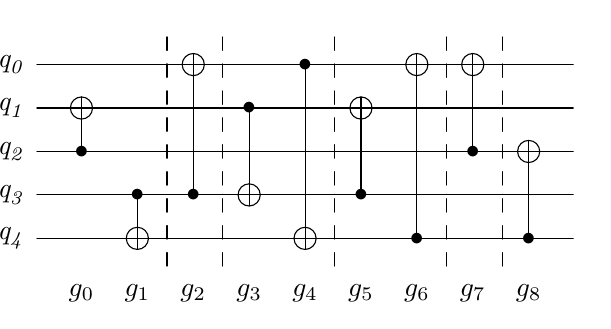
\begin{tikzpicture}
		% \draw[help lines] (0,0) grid (11,7);
		% IBM Q20
		\node at (5.5,5){  \Qcircuit @C=1.2em @R=0.75em {
			\lstick{\textit{q}_\textit{0}}   &  \qw 				&   \qw  \barrier{4}&\targ 	\barrier{4}	&\qw      		&\ctrl{4}\barrier{4}&   \qw		&\targ\barrier{4} &\targ  \barrier{4}&\qw  &  \qw       \\
			\lstick{\textit{q}_\textit{1}}   &   \targ      		&   \qw      		&   \qw      		&   \ctrl{2} 	&   \qw      	&   \targ    	&   \qw      	&   \qw       	&   \qw   		&  \qw       \\
			\lstick{\textit{q}_\textit{2}}   &   \ctrl{-1}  		&   \qw      		&   \qw      		&   \qw      	&   \qw      	&   \qw      	&   \qw     	&   \ctrl{-2} 	&   \targ       &  \qw       \\
			\lstick{\textit{q}_\textit{3}}   &\qw					&   \ctrl{1}   		&   \ctrl{-3} 		&   \targ    	&   \qw      	&   \ctrl{-2}	&   \qw      	&   \qw       	&   \qw        	&  \qw         \\
			\lstick{\textit{q}_\textit{4}}   &		\qw				& \targ				& \qw 				&   \qw      	&   \targ    	&   \qw      	&   \ctrl{-4}  	& 	\qw     	&   \ctrl{-2} 	&   \qw			\\
							  &\dstick{g_{0}}		&\dstick{g_{1}}		&\dstick{g_{2}}		&\dstick{g_{3}}	&\dstick{g_{4}} &\dstick{g_{5}} &\dstick{g_{6}} &\dstick{g_{7}} &\dstick{g_{8}}	&   		\\		 
							 &						&					&				&       		& 				& 				& 				&				&   				 
							 }};
	\end{tikzpicture}
	}					 
	\caption{A quantum circuit}
	\label{OriginalCircuit}	
	\end{center}
\end{figure}

%} %endofleaveout 15

%\paragraph{Architectures}
In the current work, we mainly consider the physical circuits of the IBM Q series.
Let $\mathcal{\mathcal{AG}_{P}}=(V_{P}, E_{P})$ denote the architecture graph of a physical circuit,
where $V_{P}$ denotes the set of physical qubits and $E_{P}$ denotes the set of edges that connect CNOT gates.
In Fig.~\ref{IBM}, diagrams (a) and (b) are the physical architecture graphs of the 5-qubit IBM QX2 and IBM QX4, respectively; diagrams (c) and (d) are the physical architecture graphs of the 16-qubit IBM QX3 and IBM QX5, respectively; diagram (e) is the physical architecture graph of IBM Q20.
The direction in each edge indicates the control direction of a 2-qubit gate,
and 2-qubit gates can only be performed between qubits with edges connected.
IBM physical circuits only support single quantum gates and CNOT gates between two adjacent qubits.
\leaveout{ %10
	 \begin{figure}[htbp]
		\begin{center}
	{\scalefont{1.0}
		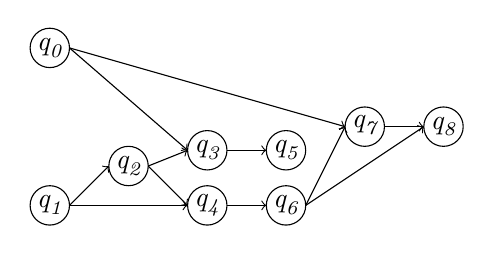
\begin{tikzpicture}							 
	\draw [black,  thin] (3,1) circle [radius=0.25];
	\draw [black,  thin] (3,3) circle [radius=0.25];
	\draw [black,  thin] (4,1.5) circle [radius=0.25];
	\draw [black,  thin] (5,1) circle [radius=0.25];
	\draw [black,  thin] (5,1.7) circle [radius=0.25];
	\draw [black,  thin] (6,1.7) circle [radius=0.25];
	\draw [black,  thin] (6,1) circle [radius=0.25];
	\draw [black,  thin] (7,2) circle [radius=0.25];
	\draw [black,  thin] (8,2) circle [radius=0.25];
	% label
	\node at (3,1) {$\textit{q}_\textit{1}$};
	\node at (3,3) {$\textit{q}_\textit{0}$};
	\node at (4,1.5) {$\textit{q}_\textit{2}$};
	\node at (5,1){$\textit{q}_\textit{4}$};
	\node at (5,1.7) {$\textit{q}_\textit{3}$};
	\node at (6,1.7){$\textit{q}_\textit{5}$};
	\node at (6,1) {$\textit{q}_\textit{6}$};
	\node at (7,2) {$\textit{q}_\textit{7}$};
	\node at (8,2) {$\textit{q}_\textit{8}$};

	% q1
	\draw [->, thin] (3.25,1) -- (3.75,1.5);
	\draw [->, thin] (3.25,1) -- (4.75,1);
	% q0
	\draw [->, thin] (3.25,3) -- (4.75,1.7);
	\draw [->, thin] (3.25,3) -- (6.75,2);
	% q2
	\draw [->, thin] (4.25,1.5) -- (4.75,1);
	\draw [->, thin] (4.25,1.5) -- (4.75,1.7);
	% q3
	\draw [->, thin] (5.25,1.7) -- (5.75,1.7);
	% q4
	\draw [->, thin] (5.25,1) -- (5.75,1);
	% q6
	\draw [->, thin] (6.25,1) -- (7.75,2);
	\draw [->, thin] (6.25,1) -- (6.75,2);
	% q7
	\draw [->, thin] (7.25,2) -- (7.75,2);
	\end{tikzpicture}
}
\end{center}
	\caption{The directed acyclic graph ($DAG$) of original circuit in Fig.~\ref{OriginalCircuit}.}
	\label{DAG}
\end{figure}
} % endofleaveout 10

\begin{figure}[htbp]
	\begin{center}
		{\scalefont{1.0}
	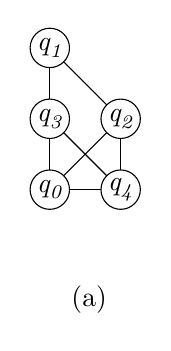
\begin{tikzpicture}
		% \tikzstyle{every node}=[font=\small,scale=0.9]

		\node at (0.5,0){(a)};
            % Q20
            \draw [black, thin] (0,1.4) circle [radius=0.25];
            \draw [-,thin] (0.25,1.4) -- (0.65,1.4);
            \draw [black, thin] (0.9,1.4) circle [radius=0.25];
            % label
            \node at (0,1.4) {$\textit{q}_\textit{0}$};
            \node at (0.9,1.4){$\textit{q}_\textit{4}$};
            % |
            \draw [-,thin] (0,1.65) -- (0,2.05);
            \draw [-,thin] (0.9,1.65)-- (0.9,2.05);
        
            \draw [black, thin] (0,2.3) circle [radius=0.25];
        
            \draw [black, thin] (0.9,2.3) circle [radius=0.25];
            % label
            \node at (0,2.3) {$\textit{q}_\textit{3}$};
            \node at (0.9,2.3){$\textit{q}_\textit{2}$};
            % |
            \draw [-,thin] (0,2.55) -- (0,2.95);
        
            \draw [black, thin] (0,3.2) circle [radius=0.25];
            \draw [-,thin] (0.175,3.025) -- (0.725,2.475);
            % label
            \node at (0,3.2) {$\textit{q}_\textit{1}$};
            %x
			\draw [-,thin] (0.175,2.125) -- (0.725,1.575);
			\draw [-,thin] (0.175,1.575) -- (0.725,2.125);
			\label{LLAG}
			\end{tikzpicture}
			}
			\qquad   \qquad
			{
				\scalefont{0.8}
			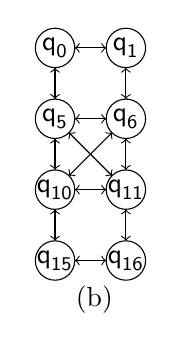
\begin{tikzpicture}
            
                % IBM Q20
            \node at (0.5,0){(b)};
            % Q20
            \draw [black, thin] (0,0.5) circle [radius=0.25];
            \draw [<->,thin] (0.25,0.5) -- (0.65,0.5);
            \draw [black, thin] (0.9,0.5) circle [radius=0.25];
        
            \node at (0,0.5) {$\textsf{q}_\textsf{15}$};
            \node at (0.9,0.5){$\textsf{q}_\textsf{16}$};
            % |
            \draw [<->,thin] (0,0.75) -- (0,1.15);
            \draw [<->,thin] (0.9,0.75) -- (0.9,1.15);
        
            \draw [black, thin] (0,1.4) circle [radius=0.25];
            \draw [<->,thin] (0.25,1.4) -- (0.65,1.4);
            \draw [black, thin] (0.9,1.4) circle [radius=0.25];
            % label
            \node at (0,1.4) {$\textsf{q}_\textsf{10}$};
            \node at (0.9,1.4){$\textsf{q}_\textsf{11}$};
            % |
            \draw [<->,thin] (0,1.65) -- (0,2.05);
            \draw [<->,thin] (0.9,1.65)-- (0.9,2.05);
        
            \draw [black, thin] (0,2.3) circle [radius=0.25];
            \draw [<->,thin] (0.25,2.3) -- (0.65,2.3);
            \draw [black, thin] (0.9,2.3) circle [radius=0.25];
            % label
            \node at (0,2.3) {$\textsf{q}_\textsf{5}$};
            \node at (0.9,2.3){$\textsf{q}_\textsf{6}$};
            % |
            \draw [<->,thin] (0,2.55) -- (0,2.95);
            \draw [<->,thin] (0.9,2.55)-- (0.9,2.95);
        
            \draw [black, thin] (0,3.2) circle [radius=0.25];
            \draw [<->,thin] (0.25,3.2) -- (0.65,3.2);
            \draw [black, thin] (0.9,3.2) circle [radius=0.25];
            % label
            \node at (0,3.2) {$\textsf{q}_\textsf{0}$};
            \node at (0.9,3.2){$\textsf{q}_\textsf{1}$};
        
            %x
        
            \draw [<->,thin] (0.175,2.125) -- (0.725,1.575);
			\draw [<->,thin] (0.175,1.575) -- (0.725,2.125);
			\label{PPAG}
	\end{tikzpicture}
			}
\end{center}
	
	\caption{(a) The architecture graph of original circuit in Fig.~\ref{OriginalCircuit}. (b) The partial architecture graph of IBM Q20.}
	\label{LAGPAG}
\end{figure}
	

Given a logical circuit $LC$, a physical structure $\mathcal{AG}_{P}$, an initial mapping $\tau$, and a CNOT gate $g=\left \langle \textit{q}_\textit{i},\textit{q}_\textit{j}\right \rangle $, where $\textit{q}_\textit{i}$ is the control qubit, $\textit{q}_\textit{j}$ is the target qubit,
if gate $g$ is executable on a physical circuit with the structure $\mathcal{AG}_{P}$, then
$\left \langle\tau(\textit{q}_\textit{i}),\tau(\textit{q}_\textit{j})\right \rangle $ 
must be a directed edge on $\mathcal{AG}_{P}$.


\begin{example}
	Fig.~\ref{LAGPAG} (a) is the logical structure of Fig.~\ref{OriginalCircuit}. 
	Fig.~\ref{LAGPAG} (b) is the partial architecture graph of IBM Q20. An initial mapping is 
	$$\tau=\{\textit{q}_\textit{0}\rightarrow  \textsf{q}_{\textsf{10}},\ \textit{q}_\textit{1}\rightarrow \textsf{q}_{\textsf{0}},\ 
	\textit{q}_\textit{2}\rightarrow  \textsf{q}_{\textsf{6}},\ \textit{q}_\textit{3}\rightarrow  \textsf{q}_{\textsf{5}},\ \textit{q}_\textit{4}\rightarrow  \textsf{q}_{\textsf{11}}\} .$$
The 2-qubit gate	$g_{0}=\left \langle \textit{q}_\textit{2},\textit{q}_\textit{1}\right \rangle $ is not executable, since the edge $\left \langle \tau(\textit{q}_\textit{2}),\tau(\textit{q}_\textit{1})\right \rangle =\left \langle \textsf{q}_{\textsf{6}},\textsf{q}_{\textsf{0}}\right \rangle $ does not exist in $\mathcal{AG}_{P}$.
	But $g_{3}=\left \langle \textit{q}_\textit{1},\textit{q}_\textit{3}\right \rangle $ is executable, since 
	the edge $\left \langle \tau(\textit{q}_\textit{1}),\tau(\textit{q}_\textit{3})\right \rangle =\left \langle \textsf{q}_{\textsf{0}},\textsf{q}_{\textsf{5}}\right \rangle $  exists in $\mathcal{AG}_{P}$.
\end{example}


\section{Quantum Circuit Transformation}
\label{Problem Description and Solution Outline}
A common assumption for circuit transformation is that we are given a circuit that has only single quantum gates and CNOT gates~\cite{1995Barenco,2005Mttnen}. We add auxiliary gates %(see Fig.~\ref{Decomposition}) 
to move two non-adjacent qubits to adjacent positions or change the direction of a CNOT gate. Adding more gates increases the risk of introducing more noise. Therefore,
we hope to find a circuit transformation algorithm that, when given an input circuit, can produce an output circuit with a minimal number of auxiliary gates and a small circuit depth in an acceptable amount of time.

Roughly speaking, quantum circuit transformation includes the following three steps.

\leaveout{ %11
\begin{figure}[htbp] 
	\centering
	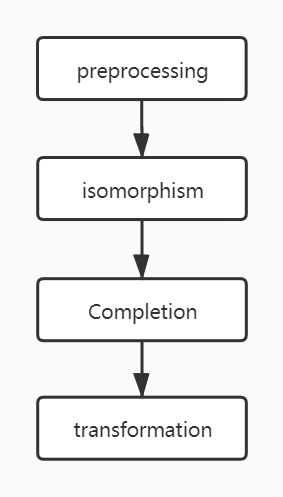
\includegraphics[scale=0.4]{uml.jpg}		 
	\caption{Circuit transformation process}
	\label{processing}	
	 \end{figure}
 } %end of leaveout 11

\begin{enumerate}
	\item \emph{Preprocessing.} 
	This step includes extracting the logical architecture graph of the circuit, adjusting the life cycle of qubits as in~\cite{2019Zhang},  and calculating the shortest paths of the physical circuit.
	\item \emph{Isomorphism and completion.} %substructures and generate a high-quality initial mapping.}
	This step uses the subgraph isomorphism algorithm to find part of the initial mapping~\cite{Sun2020}.
	Then we perform a mapping completion to include the remaining nodes that do not satisfy all isomorphism requirements, according to the connectivity between the unmapped node and the mapped nodes.
	% Unmapped nodes are mapped to the neighborhood of mapped nodes, which satisfies the connectivity of part of the logical architecture graph and physical architecture graph and reduces the length of the shortest path. 
      \item \emph{Adjustment.} %Transform logical circuits to meet physical constraints.}	Circuit transformation need to be performed before compiling quantum circuits, since the design of quantum algorithms usually does not refer to the connectivity constraints of any hardware. Therefore, it is necessary for any quantum compiler.
        After the second step, some logically adjacent nodes may be mapped to physically non-adjacent nodes, thus quantum gates applied on them cannot be executable on physical devices. It is necessary to adjust the quantum circuits by adding auxiliary gates to swap qubits. We use Tabu search for the adjustment so as to generate circuits that can be physically executed.
\end{enumerate}
Note that isomorphism and adjustment are both NP-complete~\cite{2018QubitSiraichi}. So we make use of some heuristics. Below we give a detailed account of each of the steps.

%\section{Solution Details}
%\label{Solution Details}
%Our solution includes preprocessing, isomorphism, completion, and circuit adjustment, which will be presented in turn.
\subsection{Preprocessing}
%\subsubsection{The Life Cycle of Qubits}
%Before circuit adjustment, we preprocess it by collect my data so as to shorten our search time and space. 
In the preprocessing step, we adjust the input circuit described by an openQASM program to shorten the life cycle of qubits. Then we use a Breadth-First Search (BFS) to calculate the shortest distance between each pair of nodes on the architecture graph.

We use a layered method to analyze the life cycle of qubits and pack the gates that can be executed in parallel into a $bundle$, forming a layered bundle format~\cite{2019Zhang}.
A conversion method is designed to use the layered bundle format to determine which gates can be moved so the qubits related to these gates can reduce their life cycles, and the execution time of quantum programs can also be reduced. %The algorithm reduces the error rate of quantum programs by 11\% on average. 
%In most quantum workloads, the longest qubit lifetime and the average qubit lifetime can be reduced by more than 20\%, and the execution time of some quantum programs can also be reduced.

Quantum gates acting on different qubits can be executed in parallel. Therefore, we classify the gates that can be executed in parallel into one layer, otherwise we add a new layer. The notation $L(LC)=\{\mathcal{L}_{0},\mathcal{L}_{1},...,\mathcal{L}_{n}\}$ represents the layered circuit, where $\mathcal{L}_{i} \ (0 \le i \le n) $ stands for a quantum gate set that can be executed in parallel. The quantum gate set separated by the dotted line in Fig.~\ref{OriginalCircuit} are the following $\mathcal{L}_{0}=\{g_{0},g_{1}\},\mathcal{L}_{1}=\{g_{2}\},
\mathcal{L}_{2}=\{g_{3},g_{4}\},\mathcal{L}_{3}=\{g_{5},g_{6}\},\mathcal{L}_{4}=\{g_{7}\},\mathcal{L}_{5}=\{g_{8}\}$.

At the same time of circuit layering, we generate a logical circuit architecture graph $\mathcal{AG_{L}}=(V_{L},E_{L})$, which is an undirected graph with $V_{L}$ being the set of vertices, and $E_{L}$  the set of undirected edges that represent the connectivity between qubits related by CNOT gates.
%\subsubsection{Shortest Distance}
Given a physical architecture graph and assume the distance of each edge is 1, we can use Floyd-Warshall algorithm to calculate the shortest distance matrix $dist[i][j]$, which represents the shortest distance from $\textsf{q}_{\textsf{i}}$ to $\textsf{q}_{\textsf{j}}$. 

\begin{figure}[htbp] 			
%	\centerline{ 
%		\Qcircuit @C=1.2em @R=0.5em {
%			&  \ctrl{2}  		&    \qw &   &    &  \gate{H}  		&\targ 			&\gate{H}     	&  \qw \\
%			&					&      	& 	\push{\rule{.3em}{0em}=\rule{.3em}{0em}}&	   &			& 				&	\\	 
%			&   \targ      	&    \qw 	&    &   &   \gate{H}      	&\ctrl{-2}      &\gate{H} 		&     \qw   \\	 
%			&					&      	&		   &			&				& 				&					 
%		}			
%	}
	\centerline{ 
		\Qcircuit @C=0.5em @R=0.4em {
			\lstick{\textit{q}_\textit{0}} &  \qswap  				&    \rstick{\textit{q}_\textit{1}} \qw &&&&  \lstick{\textit{q}_\textit{0}} 	&  \ctrl{2}  		&  \targ  		&  \ctrl{2}  		&    \rstick{\textit{q}_\textit{1}} \qw &&&&  \lstick{\textit{q}_\textit{0}}  &  \ctrl{2}  		&   \gate{H}  		&\ctrl{2} 			&\gate{H}     	&\ctrl{2}			&    \rstick{\textit{q}_\textit{1}}\qw  \\
			&		\qwx	&&&\push{\rule{.3em}{0em}=\rule{.3em}{0em}}&		&  	&					&			
			&		&      	& 		&	\push{\rule{.3em}{0em}=\rule{.3em}{0em}}					&					&				&					&         			&&&&			 \\
			\lstick{\textit{q}_\textit{1}} &   \qswap\qwx	   		&     \rstick{\textit{q}_\textit{0}}  \qw &&&&    \lstick{\textit{q}_\textit{1}} 	&   \targ      		&  \ctrl{-2}    &   \targ      		&     \rstick{\textit{q}_\textit{0}}  \qw   &&&&  \lstick{\textit{q}_\textit{1}}  &   \targ      		&   \gate{H}      	&   \targ      		&\gate{H} 		&\targ      		&    \rstick{\textit{q}_\textit{0}}\qw 	   \\	 
			&			&&&&		&  	&					&					&					&       		& 					&						&					&				&					&         			&&&&			 
		} 
	}
	\caption{Implenting a SWAP gate by using CNOT gates and H gates}
	\label{f:Decomposition}
\end{figure}

For IBM QX2, QX3, QX4, and QX5, the control of one qubit to a neighbour is unilateral. In this case, 
a SWAP gate can be implemented by using three CNOT gates and four H gates, as shown in Fig.~\ref{f:Decomposition}. The four H gates are needed to change the direction of the middle CNOT gate. 
Consider a CNOT gate $g=\left \langle  \textit{q}_\textit{i},\textit{q}_\textit{j} \right \rangle $. If $q_i$ and $q_j$  are mapped to $\textsf{q}_{m}$ and $\textsf{q}_{n}$, respectively, then the cost of executing $g$ under the shortest path is $cost_{cnot}(\textit{q}_\textit{i},\textit{q}_\textit{j})=7 \times( dist[m][n]-1)$. For IBM Q20, where the control between two adjacent qubits are bilateral, a SWAP gate can be implemented by using three CNOT gates. Thus the cost  is $cost_{cnot}(\textit{q}_\textit{i},\textit{q}_\textit{j})=3 \times( dist[m][n]-1)$. 
%The time complexity is $O (N^{3})$.
\begin{example}
	Take the QX5 (cf. Fig.~\ref{IBM} (d))    structure  as an example. Suppose there is a CNOT gate $g=\left \langle  \textit{q}_\textit{1}, \textit{q}_\textit{2} \right \rangle $, with \ $\textit{q}_\textit{1}$ mapped to $\textsf{q}_{1}$ and $\textit{q}_\textit{2}$ mapped to $\textsf{q}_{\textsf{14}}$. The shortest distance between them  is $dist[1][14]=3$. There are 3 shortest paths to move $\textsf{q}_{\textsf{1}}$ to an adjacent position of 
$\textsf{q}_{\textsf{14}}$:
%$\Pi=\{\pi_{0},\pi_{1},\pi_{2}\}$, 
$\pi_{0}={\textsf{q}_{\textsf{1}}\rightarrow \textsf{q}_{\textsf{2}} \rightarrow \textsf{q}_{\textsf{3}} \rightarrow \textsf{q}_{\textsf{14}}}$,
$\pi_{1}={\textsf{q}_{\textsf{1}}\rightarrow \textsf{q}_{\textsf{2}} \rightarrow \textsf{q}_{\textsf{15}} \rightarrow \textsf{q}_{\textsf{14}}}$,
$\pi_{2}={\textsf{q}_{\textsf{1}}\rightarrow \textsf{q}_{\textsf{0}} \rightarrow \textsf{q}_{\textsf{15}} \rightarrow \textsf{q}_{\textsf{14}}}$.
Their costs are given by 
$cost_{\pi_{0}}=18,\ cost_{\pi_{1}}=14,$ and $ cost_{\pi_{2}}=14$, respectively.
\end{example}

%\subsubsection{Circuit Layering}


\subsection{Isomorphism and Completion}
%It has been proved that the initial mapping has an important  influence on quantum circuit adjustment,  and the subgraph isomorphism can be reduced to initial mapping problem. Thus
%We use the subgraph isomorphism algorithm to find a partial initial mapping that promissingly minimizes auxiliary gates added by the output circuit.

%As it is known, not all logical architecture graph have a subgraph that exactly matches all the nodes in physical architecture graph.
In general, in a physical architecture graph, it is almost impossible to find a subgraph that exactly matches all the nodes in a logical architecture graph. We regard the mapping with the largest number of matching nodes as the partial mapping. SubgraphMatching compares various compositions of several state-of-the-art subgraph isomorphism algorithms.  
It shows that the best performance can be achieved by using filters and the sorting ideas of the GraphQL algorithm to process candidate nodes, and the local candidates calculation method LFTJ based on set-intersection to enumerate the results. Since SubgraphMatching cannot handle disconnected graphs, we artificially create connected graphs by connecting isolated nodes to the nodes with the largest degree in the logical architecture graph. %We would like to minimize the impact of logical dependency graphs, thus map isolated nodes to nodes with the largest degree.
\begin{algorithm}[htbp]
	\caption{Complete initial mapping}  
	\LinesNumbered  
	\KwIn{$\mathcal{AG_{L}}$: The architecture of logical circuit \\ 
	$\mathcal{AG_{P}}$: The architecture of physical circuit\\
	$T$: A partial mapping set obtained by SubgraphMatching  \\
	}
	\KwOut{$result$: A collection of mapping relations between
	 $\mathcal{AG_{L}}$ and $\mathcal{AG_{P}}$}  
	\textbf{Initialize} $result=\emptyset$ ;\\
	$l \leftarrow \max_{\tau \in T} \  \tau.length$; \\
	\For{$\tau\in T$}{
		\If{$l=\tau.length$}{
			$result.add(\tau)$;\\
			$Q \leftarrow $ an empty unmapped node queue \\
			$i \leftarrow  1$; \\ 
			\While{$i\leq \tau.length$}{
				$Q.push(\{i,\ i\leq \tau.length $ \}) \\
				$i \leftarrow i+1$;
			}
			\While{$Q\ is\ not\ empty$}{
				$\textit{q} \leftarrow Q.poll()$;\\
				$targetAdj \leftarrow$ $\mathcal{AG_{P}}.adjacencyMatrix()$; 	\\
				$queryAdj \leftarrow$ $\mathcal{AG_{L}}.adjacencyMatrix()$;	\\
				$cans \leftarrow$ an empty candidate node list sorted by degree \\
					$ cans \cup \{ \textit{q}_\textit{m}, \ \textit{q}_\textit{m} \leq queryAdj[\textit{q}].length \}$;	\\
				\While{$cans\ is\ not\ empty$}{
					$q \leftarrow \tau[cans.first]$; \\
					$k \leftarrow 0$; \\
					$cans \leftarrow cans\backslash cans.first$; \\
					\While{$ k < targetAdj[q].length$}{
						\If{  $(targetAdj[q][k]\neq -1\ or\ targetAdj[k][q]  \neq -1)$\\
						  $\ and\ not\ \tau.contains(k)$}{
							 $\tau[\textit{q}] \leftarrow k$; \\
							 break;
						 }
						  $k \leftarrow k+1$;
					}
					\If{ $k\neq targetAdj[q].length$ }{
						break;
					}
				}
			}
		}
	}
	return $result$;
	\label{algorithm_initial}
	\end{algorithm}
	
The input of Algorithm~\ref{algorithm_initial} is a target graph ($\mathcal{AG}_{P}$), a query graph ($\mathcal{AG}_{L}$), and the partial mapping set $T$. First, we initialize an empty queue $Q$.
Then we traverse $\tau$ and add the unmapped nodes to the queue $Q$. For the unmapped nodes, we try to map them to the vicinity of the mapped nodes in $\mathcal{AG}_{P}$. If a node $\textit{q}$ is not mapped to any physical node, we need to perform such kind of mapping completion. Finally, we generate a dense mapping, which can reduce the added auxiliary gates. In principle, we could try to match the remaining unmapped nodes randomly, but it may lead to a mapping with a node far away from other nodes. If an unmapped node has an edge adjacent to a matched node in the query graph, it will be matched to one of the adjacent nodes first.  In this way, we can obtain all initial candidate mappings.

% In Algorithm~\ref{algorithm_initial}, Line 2 selects the partial mapping with the most mapped nodes $l$ as the candidate set. Lines 3-28 complete the partial mapping.
% %logical qubit unmapped nodes in the candidate set.
%  In Line 6, we initialize an empty queue $Q$, which stores unmapped logical qubits. In Lines 8-10, we traverse the mapping $\tau$ and add the unmapped qubits to $Q$. We iterate the loop until $Q$ is empty, and all logical qubits are mapped to physical qubits. We take out the first element in $Q$ to \textit{q}. Lines 13-14 are used to get the adjacency matrices of $\mathcal{AG}_{P}$ and $\mathcal{AG}_{L}$, respectively. Line 15 initializes an empty map $cans$, sort by a descending order of whether $\textit{q}_\textit{m}$ is mapped and the number of gate appearances. Line 16 store the nodes $\textit{q}_\textit{m}$ connected to \textit{q} in the adjacency matrix in $ cans$. Lines 17-28 traverse  $cans$, select the node $\textit{q}_\textit{m}$ that has been mapped to the node ($cans.first$) on physical architecture graph, and  has the largest number of connections to \textit{q} in $cans$, with $ \textsf{q}$ being the node that $\textit{q}_\textit{m}$ is mapped to  in $\tau$.  Line 20 deletes the node from $cans$. Lines 21-26 select the node $k$ adjacent to \textsf{q} in the adjacency matrix, and maps \textit{q} to that node.
\begin{example}
	Following the previous example, we first use the CSIC algorithm for the logical architecture graph given in Fig.~\ref{LAGPAG} (a) and the physical architecture graph given in Fig.~\ref{IBM} (e) to obtain the partial mapping set $T=\{\tau_{0},\tau_{1},...,\tau_{n}\}$. We take one of the partial mappings as an example.
	$$\tau_{0}=\{\textit{q}_\textit{0}\rightarrow \textsf{q}_{\textsf{10}},\textit{q}_\textit{1}\rightarrow -1,
	\textit{q}_\textit{2}\rightarrow \textsf{q}_{\textsf{6}},\textit{q}_\textit{3}\rightarrow \textsf{q}_{\textsf{5}},\textit{q}_\textit{4}\rightarrow \textsf{q}_{\textsf{11}}\}. $$ 
Here $\textit{q}_\textit{1}\rightarrow -1$ means that $\textit{q}_\textit{1}$ is not mapped to any physical node, so we need to perform a mapping completion. In this example, the maximum number of mapped nodes is 4. Next, we demonstrate how $\tau_{0}$ is completed. We add all unmapped nodes to the queue $Q$. In this example, $Q=\{\textit{q}_\textit{1}\}$. Then we loop until $Q$ is empty. We pop the first element $q$ of $Q$, get the adjacency matrix of the query graph and the target graph, and traverse the adjacency matrix. We put the nodes  $\textit{q}_\textit{m}$ adjacent to \textit{q} into the candidate nodes list $cans$, which is sorted by the connectivity of $\textit{q}_\textit{m}$ and \textit{q}. We get $cans=\{\textit{q}_\textit{3},\textit{q}_\textit{2},\textit{q}_\textit{4},\textit{q}_\textit{0}\}$. Thereafter, we traverse $cans$ and take out of the first element $\textit{q}_\textit{3}$ in $cans$, and calculate the phycical node $\textsf{q}=\textsf{q}_{\textsf{5}}$, $\tau_0(\textit{q}_\textit{3})=\textsf{q}_{\textsf{5}}$. Finally, we map \textit{q} to the node connected to \textsf{q} but not yet mapped. If the nodes connected to \textsf{q} have been mapped, the loop continues. In this example, it can be directly mapped to $\textsf{q}_{\textsf{0}}$. In the end, we obtain the mapping $ \tau_{0}=\{\textit{q}_\textit{0}\rightarrow  \textsf{q}_{10},\textit{q}_\textit{1}\rightarrow \textsf{q}_{0},	\textit{q}_\textit{2}\rightarrow  \textsf{q}_{\textsf{6}},\textit{q}_\textit{3}\rightarrow  \textsf{q}_{\textsf{5}},\textit{q}_\textit{4}\rightarrow  \textsf{q}_{\textsf{11}}\}. $
	\end{example}
\subsection{Adjustment}
\subsubsection{Tabu search}
The Tabu search algorithm is a type of heuristic algorithm. It uses a tabu list to avoid searching repeated spaces, thereby avoiding deadlock. The algorithm uses amnesty rules to jump out of the local optimum to ensure the diversity of transformed results. The circuit adjustment mainly relies on the Tabu search algorithm, aiming to handle those large circuits that the current algorithm is difficult to handle and produce an output circuit closer to the optimum solution.


The following objects are defined in Tabu search: neighborhoods, neighborhood action, tabu list, candidate set, tabu object, evaluation function, and amnesty rule. All the edges that can be swapped in the current map are the neighborhoods. The tabu list avoids local optimum and guarantees the parallelism of auxiliary gates. The tabu object is the object in the tabu list. We try not to use the recently swapped qubits as much as possible, which are added to the tabu list. We perform pruning to reduce search space, because only swaps adjacent to at least one gate node are meaningful. We select the edge in the shortest path that has an intersection with the qubits contained in the gate as the candidate set. The evaluation function selects a SWAP evaluation formula from the candidate set, 
 taking the objective function as the evaluation function in general. The evaluation function should meet the requirements of some gates, 
and the number of SWAP gates added or the depth of the entire circuit should be small. The amnesty rules are used when all objects in the candidate set are banned,  or after banning an object, the target value will be greatly reduced.

\begin{algorithm} [htbp]
	\caption{Calculate the candidate sets }  
	\LinesNumbered  
	\KwIn{
	$dist$: The shortest paths of physical architecture\\
	$qubits$: The mapping from physical qubits to logical qubits \\
	$locs$: The mapping from logical qubits to physical qubits \\
	$cl$: Gates included in the current layer of circuits \\
	}
	\KwOut{$results$: The set of candidate solution }  
	\textbf{Initialize}  $results \leftarrow$ $\emptyset$;\\
					$E_{w} \leftarrow$ Calculate the weight of each edge\\
					$swap\_nodes \leftarrow $ An empty set of candidate swap nodes\\  
					
					\ForEach{ $g\in  cl$}{
						\If{$g \ is \ executable$}{
							$cl \leftarrow cl \backslash \{g\}$ ; \\
						}
						\Else{
							$\textit{q}_\textit{1} \leftarrow locs[g.control]$;\\
							$\textit{q}_\textit{2} \leftarrow locs[g.target]$;\\
							$swap\_nodes.add(\textit{q}_\textit{1});$ \\
							$swap\_nodes.add(\textit{q}_\textit{2});$ \\
						}
						
					}
					
					\ForEach{ $g\in  cl$}{
						$\textit{q}_\textit{1} \leftarrow locs[g.control]$;\\
						$\textit{q}_\textit{2} \leftarrow locs[g.target]$;\\
						\ForEach{$path \in paths[\textit{q}_\textit{1}][\textit{q}_\textit{2}]$}{
						\ForEach{$e \in path $}{
							\If{$
							\{sour\_node,\ tar\_node \}\cap swap\_nodes \neq \varnothing$}{
							$new\_qubits \leftarrow qubits$;\\
							$new\_locs  \leftarrow locs$;\\
							$\textit{q}_\textit{1} \leftarrow new\_qubits[e.source]$;\\
							$\textit{q}_\textit{2} \leftarrow new\_qubits[e.target]$;\\
							$new\_qubits[e.source]  \leftarrow  \textit{q}_\textit{2} $ ; \\
							$new\_qubits[e.target]  \leftarrow  \textit{q}_\textit{1} $;\\
							\If{$\textit{q}_\textit{1}\neq -1$}{ 
								$new\_locs[\textit{q}_\textit{1}] \leftarrow  \textit{q}_\textit{2}$;
							}
							\If{$\textit{q}_\textit{2}\neq-1$}{
								$new\_locs[\textit{q}_\textit{2}] \leftarrow  \textit{q}_\textit{1}$;
							}
							$s \leftarrow \emptyset$;\\
							$s.swaps \leftarrow p.swaps \cup \{distance.paths[path_{index}][j]\};$\\
							$s.value  \leftarrow evaluate(dist,new\_locs,cl)$;\\
							$results \leftarrow results \cup \{s\}$; \\
						}
						}
					}
					}
          return $results$;
          
	\label{algorithm_neighborhood}
	\end{algorithm}

The calculation of the neighborhoods is shown in Algorithm~\ref{algorithm_neighborhood}. The input is the current circuit mapping $\tau_{p}$. The variable $qubits$ contains the mapping of physical qubits to logical qubits, where $ j = qubits [i] $ means that the $i$-th physical qubit has been mapped to the $j$-th logical qubit. The variable $ locs $ represents the mapping of logical qubits to physical qubits, where $ j = locs [i] $ means that the $i$-th logical qubit has been mapped to the $j$-th physical qubit.
The current layer list of all gates is $cl$, and the output is a candidate set of the current mapping. The set $E$ contains the edges of all the shortest paths in the physical architecture graph of all the gates in the current layer. Lines 17-31 swap all the edges of candidate set, and calculate the cost of them.


\begin{example}
	Let us consider the mapping $$\tau_{0}=\{\textit{q}_\textit{0}\rightarrow  \textsf{q}_{\textsf{10}},\textit{q}_\textit{1}\rightarrow \textsf{q}_{\textsf{0}},
\textit{q}_\textit{2}\rightarrow  \textsf{q}_{\textsf{6}},\textit{q}_\textit{3}\rightarrow  \textsf{q}_{\textsf{5}},\textit{q}_\textit{4}\rightarrow  \textsf{q}_{\textsf{11}}\} , $$ 
for $L_{0}=\{g_{0},g_{1}\}$, $dist_{cnot}(g_{0})=3$ and $dist_{cnot}(g_{1})=3$. 
Gate $g_{1}$ can be executed directly in the $\tau_{0}$ mapping, so we delete it from $L_{0}$,
but $g_{0}$ cannot be executed in the mapping $\tau_{0}$.
Thus, a circuit adjustment is required. 
Nodes that cannot be executed join the set $swap\_nodes=\{\textsf{q}_{\textsf{0}},\textsf{q}_\textsf{6}\}$.
The set of shortest paths is $paths=\{\{\textsf{q}_{\textsf{6}}\rightarrow \textsf{q}_{\textsf{1}} \rightarrow \textsf{q}_{0} \},\{\textsf{q}_\textsf{6}\rightarrow \textsf{q}_\textsf{5} \rightarrow \textsf{q}_\textsf{0} \}\}$, 
and then we traverse the shortest paths to calculate the  candidate set.
The two endpoints of an edge passed by one of the shortest paths should intersect with the swap set and join the candidate set.
The current candidate set is $\{(\textsf{q}_\textsf{6},\textsf{q}_\textsf{1}),$ $(\textsf{q}_\textsf{1},\textsf{q}_\textsf{0}),$ $(\textsf{q}_\textsf{6},\textsf{q}_\textsf{5}),$ $(\textsf{q}_\textsf{5},\textsf{q}_\textsf{0}) \}$.
\end{example}

	\begin{algorithm}[htbp]
			\caption{Tabu search }  
			\LinesNumbered  
			\KwIn{$\tau_{ini}$: The initial mapping \\
			$tl$: Tabu list 
			}
			\KwOut{$\tau_{best}$: The best mapping}  
			\textbf{Initialize}
				$\tau_{best}  \leftarrow \tau_{ini}$; \\
				$iter \leftarrow 1$ \tcp*{Number of iterations } 
			\While{$not \ mustStop(iter, \tau_{best})$}{
				$C \leftarrow \tau_{ini}.candidates()$ \tcp*{candidate set}
				\If{C is empty}{
						$break$;
					}   
				$C_{best}  \leftarrow find\_best\_candidates(C, tl)$;\\
				\If{$C_{best}\ is\ empty$}{
						$C_{best} \leftarrow find\_amnesty\_candidates(C, tl)$;
				}
					$\tau_{best} \leftarrow C_{best}$;\\
				$tl  \leftarrow tl \cup\{C_{best}.swap\}$ ;\\
				$iter \leftarrow iter+1$;
			}
      return $\tau_{best}$
      
		\label{algorithm_Tabu}
	\end{algorithm}
        
	The circuit mapping algorithm based on Tabu search takes a layered circuit and an initial mapping as input and outputs a circuit that can be executed in the specified architecture graph, as shown in Algorithm~\ref{algorithm_Tabu}. The transformed circuit mapping of each layer is used as the initial mapping of the next layer. 
	Line 1 regards the initial mapping $\tau_{ini}$ as the best mapping $\tau_{best}$. Lines 3-12 cyclically check whether all all gates in the current layer can be executed under the mapping $\tau_{ini}$. If not all the gates are executable or the number of iterations has not reached the given maximum number, the search will continue. Otherwise, the search will terminate. Line 4 gets the current mapping candidate, and Line 7 finds the best mapping in the candidate set. The mapping will first remove the overlapping elements of the candidate set and the tabu list. Then from the remaining candidates, we choose a mapping with the lowest cost. Line 9 are the amnesty rules. When the best candidate is not found, the candidate set elements are all the same as the tabu list elements. The amnesty rules select the mapping with the lowest cost in the candidate set as the best candidate mapping. Lines 10-12 update the best mapping $\tau_{best}$ and the current mapping $\tau_{curr}$, and add the SWAP performed by the best mapping to the tabu list $tl$, indicating that the SWAP has just been performed. 
	The algorithm would try to avoid re-swapping the just swapped qubits. Then it will check whether the termination condition of the algorithm is satisfied. The condition determines whether the number of iterations has reached the maximum number, or the current mapping ensures all gates in the current layer can be executed. 
\begin{example}
Let us continue the previous example. We start searching from the initial mapping. We need to get the candidate SWAP set and select the one with the lower evaluation scores.
For $L_{0}=\{g_{0},g_{1}\}$, the candidate set is 
$\{(\textsf{q}_\textsf{6},\textsf{q}_\textsf{1}), (\textsf{q}_\textsf{1},\textsf{q}_\textsf{0}), (\textsf{q}_\textsf{6},\textsf{q}_\textsf{5}), (\textsf{q}_\textsf{5},\textsf{q}_\textsf{0}) \} , $ and the costs are given as follows.
\[\begin{array}{l}
cost((\textsf{q}_\textsf{6},\textsf{q}_\textsf{1}))=3.0, \, cost((\textsf{q}_\textsf{1},\textsf{q}_\textsf{0}))=3.0,\\ cost((\textsf{q}_\textsf{6},\textsf{q}_\textsf{5}))=3.0, \, cost((\textsf{q}_\textsf{5},\textsf{q}_\textsf{0}))=3.0 .
\end{array}\]
The algorithm will choose the first SWAP, the mapping becomes $$\tau_{0}=\{\textit{q}_\textit{0}\rightarrow  \textsf{q}_\textsf{10},\textit{q}_\textit{1}\rightarrow  \textsf{q}_\textsf{0},
\textit{q}_\textit{2}\rightarrow  \textsf{q}_\textsf{1},\textit{q}_\textit{3}\rightarrow  \textsf{q}_\textsf{5},\textit{q}_\textit{4}\rightarrow  \textsf{q}_\textsf{11}\} . $$ 
 %The algorithm loops to determine whether it reachs the termination condition. 
 It can be seen that the current mapping ensures the executability of $g_{0}$. The algorithm continues to search for the next layer.
\end{example}
\subsubsection{Evaluation functions }
We can control the search direction by changing the evaluation functions.
We test two evaluation functions: one uses the number of auxiliary gates in the generated circuit as the evaluation criterion (\ref{cost_num}),  and the other uses the depth of the generated circuit as the evaluation criterion  (\ref{cost_depth}).
\begin{equation}
	 	\begin{aligned}
	cost((\textsf{q}_\textsf{m},\textsf{q}_\textsf{n}))=\sum_{g \in L}(dist[\tau(g.control)][\tau(g.target)])
    \label{cost_num}
         \end{aligned}
\end{equation}
	\begin{equation}
		cost((\textsf{q}_\textsf{m},\textsf{q}_\textsf{n}))= Depth(L)
		\label{cost_depth}
		\end{equation}
Here $cost((\textsf{q}_\textsf{m},\textsf{q}_\textsf{n}))$ represents the cost of executing all the gates of the current layer $L$ 
after swapping $\textsf{q}_\textsf{m}$ with $\textsf{q}_\textsf{n}$. We only calculate the depth between the unmapped gates as in (\ref{cost_num}) or the distance of the unmapped gates as in (\ref{cost_depth}).

\subsubsection{Look ahead }
We observe that the number of gates in each layer after layering is small. The output of the $i$-th $(i<n)$ layer is used as the input of the $(i+1)$-th layer. Note that any swap operation in the $i$-th layer will affect the mapping of the $(i+1)$-th layer. If we only consider the gates in the current layer when choosing the swapping gates, the swap only satisfies the requirement of the $i$-th layer, not necessarily the next layer. Therefore, we take the gates in the $(i+x)$-th $(i+x<n)$ layer into consideration, where $x$ is the number of forward-looking layers. However, it is necessary to give a higher priority to the execution of the gates in the $i$-th layer, so we introduce an attenuation factor $\delta$, which controls the influence of the gates in the $(i+x)$-th layer. Heuristics show that for $x=2,\ \delta=0.9$, the final effect is  approximately the best. Our evaluation functions in (\ref{cost_num}) and  (\ref{cost_depth}) can be adjusted as
(\ref{cost_num_look}) and  (\ref{cost_depth_look}), respectively.
 \begin{equation}
	 	\begin{aligned}
			cost((\textsf{q}_\textsf{m},\textsf{q}_\textsf{n}))&=\sum_{g \in L_{i}}(dist[\tau(g.control)][\tau(g.target)])+\\
	&\delta \times \sum_{j=i}^{i+x}\sum_{g \in L_{j}}(dist[\tau(g.control)][\tau(g.target)])
	\label{cost_num_look}
	\end{aligned}
 \end{equation}
	\begin{equation}
		cost((\textsf{q}_\textsf{m},\textsf{q}_\textsf{n}))= Depth(L_{i})+\delta \times Depth(\sum_{j=i}^{i+x}L_{j}).
		\label{cost_depth_look}
		\end{equation}
\subsubsection{Complexity}
Given a logical circuit architecture graph  $\mathcal{AG_{L}}=(V_{L},E_{L})$ and a physical circuit architecture graph $\mathcal{AG_{P}}=(V_{P},E_{P})$, we assume that the initial mapping is $\tau$, the depth of the circuit is $d$, and the number of qubits is $V_{L}$. Tabu search deals with one layer at a time, and searches at most $d$ times. Starting from the initial mapping, we first delete the executable gates of the first layer under the initial mapping. Then, the edges of all the shortest paths of all the gates that are not executable in the current layer are added to the candidate set where at least one node is in the gate mapping. In the worst case, the length of the shortest path  is $(|E_{P}|-1)$
and the size of the candidate set  is $(|E_{P}|-1)$. Each SWAP will make the total distance between the gates smaller. In the worst case, the number of SWAPs is $(|E_{P}|-1)^{|E_{P}|-2}$, but our selection strategy will make the number of SWAPs significantly reduced. The time complexity in the worst case is $d\times (|E_{P}|-1)^{(|E_{P}|-2)}$, and the space complexity is the size of our candidate set $(E_{P}-1)$.
\section{Experiments}
\label{Experiment}
We compare the  CSIC  algorithm 
and the circuit adjustment algorithm based on Tabu search TSA with the wghtgraph in~\cite{2020Qubit} and the heuristic algorithm $ A^{*}$  in~\cite{Zulehner2017}.
All the experiments are conducted on a Windows machine with 3.3GHz CPU and 10G memory. 
 
First, we compare the efficiency of initial mapping on optm~\cite{Zulehner2017},  CSIC and wghtgraph~\cite{2020Qubit}. In order to  observe the results of these two initial mapping algorithms, we used the same circuit adjustment algorithm $A^{*}$~\cite{Zulehner2017}.
We have tested 159 circuits. Within five minutes, optm,  wghtgraph, and CSIC can handle 121, 106, and  131 circuits, respectively. There are 103 circuits that they can handle. We then compare the wghtgraph algorithm and the CSIC algorithm more closely. The wghtgraph algorithm has 21 circuits with fewer auxiliary gates  and 19 circuits with smaller depths, and the CSIC algorithm has 54 circuits with fewer auxiliary gates and 60 circuits with  smaller depths. They output 25 circuits with equal depth and  29 circuits with equal auxiliary gates. On average, the auxiliary gates of the CSIC algorithm are reduced by 22.44\%, 
and the depths are reduced by 11.25\%.
\begin{table*}[htbp]
	\begin{center}  
	\begin{tabular}{|c|c|c|c|c|c|}
	\hline
	    	&  optm & wgtgraph &CSIC & CSIC /optm & CSIC /wgtgraph\\
	\hline
	 Depths 	&	168895	&   163422	&  145040 	& 14.12\%  &11.25\%   \\
	\hline
	 Auxiliary gates 	&	20439	&  19232 	&  14916 & 27.02\% 	&  22.44\%  \\
	\hline
	\end{tabular} 
	\end{center} 
	\caption{Comparison of optm, wgtgraph and CSIC}
	\label{tab1}
	\end{table*}
  \begin{table*}[htbp]
   \begin{center}
   \begin{tabular}{|p{1.7cm}<{\centering}|p{1cm}<{\centering}|p{1cm}<{\centering}|p{1cm}<{\centering}|p{1cm}<{\centering}|p{1cm}<{\centering}|p{1cm}<{\centering}|p{1cm}<{\centering}|p{1cm}<{\centering}|p{1.2cm}<{\centering}|}
   \hline
   \multirow{2}*{benchmarks}&\multirow{2}*{\#circ.}&\multicolumn{2}{c|}{TSA$_{num}$}&\multicolumn{2}{c|}{TSA$_{dep}$} & \multicolumn{2}{c|}{wgtgraph} & \multicolumn{2}{c|}{SABRE} \\
     \cline{3-10}		
   &&\#succ.&time&\#succ.&time&\#succ.&time&\#succ.&time\\
   \hline
   small&66&66&32&66&29&64&587&23&12996\\
   \hline
   medium&49&49&45&49&40&35&1183&6&13019\\
   \hline
   large&44&44&407&44&432&0&-&0&1340719\\
   \hline
   total&159&159&484&159&501&99&-&29&1366734\\
   \hline
   \end{tabular}
   \end{center} 
   \caption{Comparison of TSA$_{num}$, TSA$_{dep}$, wghtgraph and SABRE}
   \label{tabextra}
   \end{table*}
Next, we compare the optm algorithm with the CSIC algorithm. The optm algorithm has one circuit with fewer auxiliary gates and two circuits with a small depth, while the CSIC algorithm has 99 circuits with fewer auxiliary gates and 98 circuits with a small depth.  
They have 4 circuits with equal depth and 4 circuits with equal auxiliary gates. The auxiliary gates of the CSIC algorithm are relatively reduced by 27.02\%, and the depths are reduced by 14.12\%. Table~\ref{tab1} shows the experimental data on 104 circuits. The three initial mapping algorithms are compared according to the depths of the generated circuits using the same $A^{*}$ algorithm, and the numbers of added auxiliary gates. The column headed by CSIC /optm  shows the efficiency improvement of the former upon the latter $(n_{optm}-n_{CSIC })/n_{optm}$.


	We then compare in Table~\ref{tabextra} the use of two indicators TSA$_{dep}$ and TSA$_{num}$ that prioritize smaller depths and fewer auxiliary gates, respectively. Using the two indicators  as objective functions, we tested 159 circuits. The depths of the final circuits obtained by TSA$_{num}$ are 1.93\% smaller than TSA$_{dep}$ on average, and the numbers of auxiliary gates added are 4.53\% smaller on average. When inserting a SWAP gate, the circuit needs to add 3 CNOT gates, and the depth will be increased by 3.  Therefore, if fewer SWAP gates are added, the depths of the circuits will reduce accordingly. 
	%Thus we use SWAP quantity first to give better results. 

	Finally, we compare TSA with wgtgraph.  Since the wgtgraph algorithm only uses 2-qubit gates, 
	it is impossible to compare the depths of the generated circuits.  Instead, we compare the number of SWAP gates added and the time costs. 
	%Since large circuits may not successfully handle for a long time, we consider it meaningless.  
  We set a five-minute timeout period and tested 159 circuits. It turns out that TSA$_{num}$ only takes 461 seconds and TSA$_{dep}$ takes 485 seconds. The  wgtgraph algorithm takes 1908 seconds for the 159 circuts,  but only produces valid results for 99 circuits, including 64 small circuits,  35 medium-sized circuits,  and no circuit output is produced for any of the 44 large circuits. Although Tabu search can quickly produce results on large circuits, in contrast,  more auxiliary gates are added.  In the generated circuits obtained by wgtgraph from  99 small and medium-sized circuits,  the number of SWAP gates added by wgtgraph is 26.87\% (resp. 24.89\%) smaller than TSA$_{num}$ (resp. TSA$_{dep}$) on average. The Tabu search can quickly output converted circuits on large circuits, but wgtgraph cannot get results in the predefined time bound. Since  our candidate set is too small to be able to process the circuit quickly, but this also leads to an increase in the insertion of additional gates. As to SABRE, when dealing with 159 circuits with a five-minute limit for each circuit, it successfully produces results for only 23 small circuits, 6 medium-sized circuits, and 1 large circuit. The detailed results of the circuit comparisons are in the Appendices. 
  
  \section{Conclusion}
  \label{Conclusion}
  We propose a scalable algorithm for quantum circuit transformation. First, we use a subgraph isomorphism algorithm and a mapping completion method based on the connectivity between qubits to generate a high-quality initial mapping. Secondly we exploit a look-ahead heuristic search taking into account the influence of the pre-layer circuit mapping to reduce the number of auxiliary gates, and complete the transformation. Finally, we compare the influence of initial mapping  with the state-of-the-art algorithm wghtgraph and optm and also compare the overall efficiency with optm, wghtgraph, and SABRE.
  Experimental results show that the initial mapping generated by CSIC have fewer SWAP gates inserted and the results can be obtained in an acceptable amount of time. Most small and medium-sized circuits can be handled in a few seconds.
  For large circuits, the results can be obtained within a few minutes,
  but the cost of insertion may be lareger than that of wgtgraph.
  We introduce a look-ahead method to make each selected SWAP more in line with the constraints of the gates to be processed.
  In the future, we will investigate how to reduce the number of inserted auxiliary gates  and increase the speed. We will also apply the proposed method to more NISQ devices.
  %We would introduce quantum noise to the circuits, since our simulate circuits ignore the noise generated by the circuit.

\bibliographystyle{IEEEtran}
\bibliography{IEEEabrv,mybibfile}
\appendices
\section{Experimental details of the added SWAP gate and depth of the output circuit}
The qubit no. indicates the number of qubits in the circuit, the CNOT no. indicates the number of initial CNOT gates, TSA$_{num}$, TSA$_{dep}$, optm, wghtgr, SABRE indicate the number of CNOT gates added by the TSA using their respective circuit transformation methods. Since wghtgr and SABRE do not count the depth of the converted circuit, no comparison is made. "-" means that the circuit cannot be successfully transformed within five minutes.

Table \RNum{3} and Table \RNum{4} show the circuits that TSA$_{num}$, TSA$_{dep}$, optm, wghtgr can successfully transform, and calculate the total number of gates added by them. Table \RNum{5} shows the circuits that optm, wghtgr, and SABRE may not be able to handle. Table \RNum{6} \RNum{7} shows the depth of the circuit after TSA$_{num}$, TSA$_{dep}$, optm can be successfully transform.  Table \RNum{8} shows the circuits that optm cannot handle.

\begin{table*}[htbp]
    \begin{center}  
    \begin{tabular}{|p{4.3cm}<{\centering}|c|c|c|c|c|c|c|}
    \hline
    Circuit &  qubit  & CNOT &TSA$_{num}$& TSA$_{dep}$  & optm 	 & wghtgr  &SABRE 	\\
     name	&   no. 	&	no. & added&  added &  added 	&  added&  added\\
    \hline
    decod24-enable\_126 & 6 & 149 & 28 & 42 & 60 & 16 &129\\ 
4mod5-v0\_19 & 5 & 16 & 0 & 0 & 0 & 0&- \\ 
4mod5-v0\_18 & 5 & 31 & 2 & 5 & 4 & 4 &-\\ 
mod5d2\_64 & 5 & 25 & 5 & 6 & 8 & 3&- \\ 
4gt4-v0\_72 & 6 & 113 & 14 & 10 & 33 & 14&- \\ 
alu-v3\_35 & 5 & 18 & 2 & 4 & 8 & 2 &-\\ 
4gt4-v0\_73 & 6 & 179 & 27 & 34 & 76 & 12&- \\ 
alu-v3\_34 & 5 & 24 & 2 & 3 & 7 & 2& - 	\\
3\_17\_13 & 3 & 17 & 0 & 0 & 6 & 0& 0 	\\
4gt4-v0\_78 & 6 & 109 & 12 & 8 & 48 & 4& 124 	\\
4gt4-v0\_79 & 6 & 105 & 17 & 17 & 48 & 3& - 	\\
4mod7-v1\_96 & 5 & 72 & 16 & 19 & 27 & 7& - 	\\
mod10\_171 & 5 & 108 & 17 & 20 & 39 & 9& - 	\\
ex2\_227 & 7 & 275 & 48 & 59 & 121 & 33& - 	\\
mod10\_176 & 5 & 78 & 14 & 14 & 38 & 8& - 	\\
0410184\_169 & 5 & 9 & 2 & 2 & 49 & 3& - 	\\
4mod5-v0\_20 & 5 & 10 & 0 & 0 & 4 & 0& - 	\\
aj-e11\_165 & 5 & 69 & 8 & 8 & 33 & 7& 63 	\\
alu-v1\_28 & 5 & 18 & 2 & 4 & 11 & 2& - 	\\
4gt12-v0\_86 & 6 & 116 & 28 & 33 & 48 & 3& - 	\\
4gt12-v0\_87 & 6 & 112 & 27 & 32 & 45 & 2& - 	\\
4gt12-v0\_88 & 6 & 86 & 5 & 5 & 25 & 4& - 	\\
alu-v1\_29 & 5 & 17 & 4 & 4 & 11 & 2& 13 	\\
ham7\_104 & 7 & 149 & 28 & 34 & 68 & 12& - 	\\
C17\_204 & 7 & 205 & 26 & 53 & 99 & 22& - 	\\
xor5\_254 & 6 & 5 & 0 & 0 & 1 & 0& 3	\\
hwb4\_49 & 5 & 107 & 14 & 15 & 38 & 11& 157 	\\
rd73\_140 & 10 & 104 & 23 & 26 & 35 & 20& - 	\\
decod24-v0\_38 & 4 & 23 & 0 & 0 & 6 & 0& - 	\\
rd53\_131 & 7 & 200 & 39 & 39 & 98 & 24& - 	\\
rd53\_133 & 7 & 256 & 37 & 47 & 102 & 27& 160 	\\
rd53\_135 & 7 & 134 & 28 & 29 & 38 & 23& - 	\\
decod24-v2\_43 & 4 & 22 & 0 & 0 & 9 & 0& 39 \\
rd53\_138 & 8 & 60 & 14 & 16 & 23 & 9& - \\
rd32-v0\_66 & 4 & 16 & 0 & 0 & 6 & 0& - \\
4gt13-v1\_93 & 5 & 30 & 0 & 0 & 13 & 0& - \\
graycode6\_47 & 6 & 5 & 0 & 0 & 0 & 0& - \\
4mod5-bdd\_287 & 7 & 31 & 3 & 6 & 8 & 6& 34 \\
ham3\_102 & 3 & 11 & 0 & 0 & 3 & 0& 12 \\
4gt4-v0\_80 & 6 & 79 & 5 & 5 & 22 & 5& - \\
ex-1\_166 & 3 & 9 & 0 & 0 & 3 & 0& - \\
mod5mils\_65 & 5 & 16 & 0 & 0 & 6 & 0& - \\
0example & 5 & 9 & 1 & 2 & 3 & 3& - \\
alu-v4\_36 & 5 & 51 & 12 & 8 & 22 & 4& 41 \\
alu-v4\_37 & 5 & 18 & 2 & 4 & 8 & 2& - \\
ex1\_226 & 6 & 5 & 0 & 0 & 1 & 0& 15 \\
one-two-three-v0\_98 & 5 & 65 & 11 & 13 & 32 & 10& - \\
one-two-three-v0\_97 & 5 & 128 & 23 & 23 & 64 & 16& - \\
one-two-three-v3\_101 & 5 & 32 & 3 & 4 & 14 & 3& - \\
rd32\_270 & 5 & 36 & 3 & 3 & 6 & 6 &24\\
        rd53\_130 & 7 & 448 & 89 & 100 & 190 & 49& - \\
rd53\_251 & 8 & 564 & 104 & 131 & 230 & 45& - \\
4mod5-v1\_24 & 5 & 16 & 0 & 0 & 3 & 0& - \\
mod5adder\_127 & 6 & 239 & 21 & 56 & 111 & 20& - \\
4\_49\_16 & 5 & 99 & 20 & 17 & 40 & 10& - \\
hwb5\_53 & 6 & 598 & 141 & 168 & 173 & 59& - \\
ex3\_229 & 6 & 175 & 10 & 9 & 50 & 11& - \\
4gt10-v1\_81 & 5 & 66 & 14 & 15 & 28 & 6& - \\
alu-v2\_32 & 5 & 72 & 15 & 17 & 27 & 7& - \\
alu-v2\_31 & 5 & 198 & 42 & 54 & 85 & 13& - \\
alu-v2\_30 & 6 & 223 & 41 & 45 & 96 & 20& - \\
sf\_276 & 6 & 336 & 12 & 52 & 138 & 12& - \\
decod24-v1\_41 & 5 & 38 & 4 & 4 & 14 & 3& 28 \\
sf\_274 & 6 & 336 & 34 & 21 & 82 & 12& - \\
4gt4-v1\_74 & 6 & 119 & 17 & 24 & 37 & 9& - \\
alu-v2\_33 & 5 & 17 & 4 & 4 & 8 & 2& - \\
cnt3-5\_179 & 16 & 85 & 6 & 6 & 35 & 4& - \\
\hline
    \end{tabular} 
    \end{center}
    \caption{Comparison of  the numbers of SWAP gates added by the 
    output circuits on the IBM Q20 } 
    \label{tab2}
    \end{table*}

    \begin{table*}[htbp]
        \begin{center}  
        \begin{tabular}{|p{4.3cm}<{\centering}|c|c|c|c|c|c|c|}
        \hline
        Circuit &  qubit  & CNOT &TSA$_{num}$& TSA$_{dep}$  & optm 	 & wghtgr  &SABRE 	\\
         name	&   no. 	&	no. & added&  added &  added 	&  added &  added\\
        \hline
decod24-v1\_41 & 5 & 38 & 4 & 4 & 14 & 3& 28 \\
sf\_274 & 6 & 336 & 34 & 21 & 82 & 12& - \\
4gt4-v1\_74 & 6 & 119 & 17 & 24 & 37 & 9& - \\
alu-v2\_33 & 5 & 17 & 4 & 4 & 8 & 2& - \\
cnt3-5\_179 & 16 & 85 & 6 & 6 & 35 & 4& - \\
4mod5-v1\_22 & 5 & 11 & 0 & 0 & 5 & 0&0 \\
4mod5-v1\_23 & 5 & 32 & 5 & 5 & 4 & 3& 55\\
mini\_alu\_305 & 10 & 77 & 10 & 20 & 28 & 8& 123 \\
alu-v0\_26 & 5 & 38 & 7 & 10 & 13 & 3& - \\
alu-bdd\_288 & 7 & 38 & 4 & 12 & 16 & 6& - \\
alu-v0\_27 & 5 & 17 & 2 & 4 & 11 & 2& 9 \\
4gt13\_91 & 5 & 49 & 7 & 7 & 10 & 2& - \\
4gt5\_77 & 5 & 58 & 12 & 12 & 20 & 6& - \\
4gt13\_92 & 5 & 30 & 0 & 0 & 14 & 0& - \\
            4gt5\_76 & 5 & 46 & 7 & 10 & 24 & 5&39 \\
            4gt5\_75 & 5 & 38 & 5 & 12 & 16 & 4& 53 \\
            4gt12-v1\_89 & 6 & 100 & 11 & 21 & 38 & 4& - \\
            4gt11\_83 & 5 & 14 & 0 & 0 & 0 & 0& - \\
            mod5d1\_63 & 5 & 13 & 0 & 0 & 1 & 0& - \\
            4gt11\_82 & 5 & 18 & 1 & 1 & 1 & 1& - \\
            decod24-v3\_45 & 5 & 64 & 15 & 15 & 32 & 8& 64 \\
            rd32-v1\_68 & 4 & 16 & 0 & 0 & 6 & 0& 24 \\
            mini-alu\_167 & 5 & 126 & 27 & 27 & 49 & 11& - \\
            one-two-three-v2\_100 & 5 & 32 & 3 & 4 & 8 & 3& - \\
            4mod7-v0\_94 & 5 & 72 & 8 & 13 & 36 & 9& - \\
            cm82a\_208 & 8 & 283 & 41 & 69 & 84 & 33& - \\
            mod8-10\_178 & 6 & 152 & 5 & 20 & 13 & 7& - \\
            mod8-10\_177 & 6 & 196 & 14 & 33 & 58 & 13& 230 \\
            majority\_239 & 7 & 267 & 39 & 43 & 105 & 33& - \\
            miller\_11 & 3 & 23 & 0 & 0 & 9 & 0& 36 \\
            decod24-bdd\_294 & 6 & 32 & 4 & 4 & 9 & 4& 36 \\
            \hline
            total & 551 & 9244 & 1372 & 1738 & 3481 & 800 &-\\
        \hline
        \end{tabular} 
        \end{center} 
        \caption{Comparison of the numbers of SWAP gates added by the 
        output circuits on the IBM Q20 } 
        \label{tab3}
        \end{table*}	

        \begin{table*}[htbp]
            \begin{center}  
            \begin{tabular}{|p{4.3cm}<{\centering}|c|c|c|c|c|c|c|}
            \hline
            Circuit &  qubit  & CNOT &TSA$_{num}$& TSA$_{dep}$  & optm 	 & wghtgr  &SABRE 	\\
             name	&   no. 	&	no. & added&  added &  added 	&  added&  added\\
            \hline
            max46\_240 & 10 & 11844 & 3473 & 4545 & - & -& - \\
rd73\_252 & 10 & 2319 & 586 & 761 & - & -& - \\
cycle10\_2\_110 & 12 & 2648 & 919 & 1216 & 961 & -& - \\
sqrt8\_260 & 12 & 1314 & 379 & 492 & 457 & -& - \\
urf4\_187 & 11 & 224028 & 54785 & 60140 & - & -& - \\
sqn\_258 & 10 & 4459 & 1199 & 1420 & - & -& - \\
f2\_232 & 8 & 525 & 87 & 124 & 218 & -& - \\
radd\_250 & 13 & 1405 & 386 & 489 & 511 & -& - \\
ham15\_107 & 15 & 3858 & 1326 & 1689 & - & -& - \\
sao2\_257 & 14 & 16864 & 5346 & 7178 & - & -& - \\
sym9\_148 & 10 & 9408 & 1865 & 2432 & - & -& - \\
urf5\_280 & 9 & 23764 & 6989 & 8730 & - & -& - \\
square\_root\_7 & 15 & 3089 & 812 & 2150 & - & -& - \\
sys6-v0\_111 & 10 & 98 & 23 & 26 & 38 & -& - \\
hwb7\_59 & 8 & 10681 & 2687 & 3551 & 3722 & -& - \\
sym9\_146 & 12 & 148 & 38 & 55 & 54 & -& 248 \\
wim\_266 & 11 & 427 & 93 & 120 & 147 & -& - \\
urf2\_152 & 8 & 35210 & 9181 & 11921 & 10577 & -& - \\
urf5\_159 & 9 & 71932 & 20258 & 25505 & - & -& - \\
urf2\_277 & 8 & 10066 & 2807 & 3798 & 3782 & -& - \\
life\_238 & 11 & 9800 & 2762 & 3576 & - & -& - \\
root\_255 & 13 & 7493 & 2128 & 3035 & - & -& - \\
9symml\_195 & 11 & 15232 & 4553 & 5986 & - & -& - \\
sym10\_262 & 12 & 28084 & 8534 & 11033 & - & -& - \\
dc1\_220 & 11 & 833 & 226 & 207 & 371 & -& - \\
cm42a\_207 & 14 & 771 & 182 & 229 & 294 & -& - \\
rd53\_311 & 13 & 124 & 26 & 48 & 47 & -& - \\
dc2\_222 & 15 & 4131 & 1383 & 1773 & - & -& - \\
rd84\_142 & 15 & 154 & 49 & 58 & 50 & -& - \\
sym6\_145 & 7 & 1701 & 317 & 449 & 750 & -& - \\
co14\_215 & 15 & 7840 & 3078 & 3819 & - & -& - \\
cnt3-5\_180 & 16 & 215 & 59 & 74 & 79 & -& - \\
cm152a\_212 & 12 & 532 & 103 & 129 & 168 & -& - \\
sym6\_316 & 14 & 123 & 30 & 39 & 56 & -& - \\
mlp4\_245 & 16 & 8232 & 2780 & 3490 & - & -& - \\
hwb8\_113 & 9 & 30372 & 10749 & 16489 & - & -& - \\
qft\_16 & 16 & 240 & 90 & 147 & - & -& - \\
plus63mod4096\_163 & 13 & 56329 & 19759 & 24273 & - & -& - \\
urf1\_149 & 9 & 80878 & 22551 & 28516 & - & -& - \\
urf3\_155 & 10 & 185276 & 50842 & 62903 & - & -& - \\
urf3\_279 & 10 & 60380 & 17999 & 23318 & - & -& - \\
hwb9\_119 & 10 & 90955 & 22946 & 30031 & - & -& - \\
plus63mod8192\_164 & 14 & 81865 & 28022 & 36207 & - & -& - \\
pm1\_249 & 14 & 771 & 182 & 229 & 294 & -& - \\
sym9\_193 & 11 & 15232 & 4382 & 5518 & - & -& - \\
misex1\_241 & 15 & 2100 & 480 & 754 & 600 & -& - \\
urf1\_278 & 9 & 26692 & 8010 & 10217 & - & -& - \\
squar5\_261 & 13 & 869 & 219 & 313 & 290 & -& - \\
ground\_state\_estimation\_10 & 13 & 154209 & 11671 & 22886 & - & -& - \\
adr4\_197 & 13 & 1498 & 516 & 670 & - & -& - \\
hwb6\_56 & 7 & 2952 & 698 & 933 & 909 & -& - \\
clip\_206 & 14 & 14772 & 5430 & 6865 & - & -& - \\
cm85a\_209 & 14 & 4986 & 2088 & 2225 & - & -& - \\
rd84\_253 & 12 & 5960 & 1849 & 2333 & - & -& - \\
dist\_223 & 13 & 16624 & 5623 & 7431 & - & -& - \\
inc\_237 & 16 & 4636 & 1193 & 1667 & - & -& - \\
qft\_10 & 10 & 90 & 23 & 34 & 30 & -& - \\
urf6\_160 & 15 & 75180 & 27524 & 32452 & - & -& - \\
con1\_216 & 9 & 415 & 86 & 118 & 177 & -& - \\
            \hline
            \end{tabular} 
            \end{center}	
            \caption{Comparison of  the numbers of SWAP gates added by the 
            output circuits on the IBM Q20 }
            \label{tab4}  
            \end{table*}
              
\begin{table*}[htbp]
    \begin{center}  
        \begin{tabular}{|p{4.3cm}<{\centering}|c|c|c|c|c|c|}
            \hline
                        Circuit &  qubit  & CNOT &depths &TSA$_{num}$& TSA$_{dep}$  & optm 	  	\\
                         name	&   no. 	&	no. & no. & depths&  depths &  depths 	\\
                        \hline
                        decod24-enable\_126 & 6 & 149 & 190 & 233 & 275 & 470 \\
4mod5-v0\_19 & 5 & 16 & 21 & 16 & 16 & 21 \\
4mod5-v0\_18 & 5 & 31 & 40 & 37 & 46 & 54 \\
mod5d2\_64 & 5 & 25 & 32 & 40 & 43 & 67 \\
4gt4-v0\_72 & 6 & 113 & 137 & 155 & 143 & 297 \\
alu-v3\_35 & 5 & 18 & 22 & 24 & 30 & 60 \\
4gt4-v0\_73 & 6 & 179 & 227 & 260 & 281 & 586 \\
alu-v3\_34 & 5 & 24 & 30 & 30 & 33 & 63 \\
3\_17\_13 & 3 & 17 & 22 & 17 & 17 & 52 \\
4gt4-v0\_78 & 6 & 109 & 137 & 145 & 133 & 352 \\
4gt4-v0\_79 & 6 & 105 & 132 & 156 & 156 & 345 \\
4mod7-v1\_96 & 5 & 72 & 94 & 120 & 129 & 218 \\
mod10\_171 & 5 & 108 & 139 & 159 & 168 & 335 \\
ex2\_227 & 7 & 275 & 355 & 419 & 452 & 899 \\
mod10\_176 & 5 & 78 & 101 & 120 & 120 & 104 \\
cycle10\_2\_110 & 12 & 2648 & 3386 & 5405 & 6296 & 7467 \\
0410184\_169 & 5 & 9 & 6 & 15 & 15 & 253 \\
4mod5-v0\_20 & 5 & 10 & 12 & 10 & 10 & 32 \\
sqrt8\_260 & 12 & 1314 & 1661 & 2451 & 2790 & 3561 \\
aj-e11\_165 & 5 & 69 & 86 & 93 & 93 & 250 \\
alu-v1\_28 & 5 & 18 & 22 & 24 & 30 & 70 \\
f2\_232 & 8 & 525 & 668 & 786 & 897 & 1672 \\
radd\_250 & 13 & 1405 & 1781 & 2563 & 2872 & 3985 \\
4gt12-v0\_86 & 6 & 116 & 135 & 200 & 215 & 334 \\
4gt12-v0\_87 & 6 & 112 & 131 & 193 & 208 & 324 \\
4gt12-v0\_88 & 6 & 86 & 108 & 101 & 101 & 222 \\
alu-v1\_29 & 5 & 17 & 22 & 29 & 29 & 64 \\
ham7\_104 & 7 & 149 & 185 & 233 & 251 & 491 \\
C17\_204 & 7 & 205 & 253 & 283 & 364 & 688 \\
xor5\_254 & 6 & 5 & 5 & 5 & 5 & 10 \\
hwb4\_49 & 5 & 107 & 134 & 149 & 152 & 308 \\
rd73\_140 & 10 & 104 & 92 & 173 & 182 & 185 \\
decod24-v0\_38 & 4 & 23 & 30 & 23 & 23 & 61 \\
rd53\_131 & 7 & 200 & 261 & 317 & 317 & 677 \\
rd53\_133 & 7 & 256 & 327 & 367 & 397 & 777 \\
rd53\_135 & 7 & 134 & 159 & 218 & 221 & 331 \\
sys6-v0\_111 & 10 & 98 & 75 & 167 & 176 & 188 \\
decod24-v2\_43 & 4 & 22 & 30 & 22 & 22 & 75 \\
hwb7\_59 & 8 & 10681 & 13437 & 18742 & 21334 & 29601 \\
rd53\_138 & 8 & 60 & 56 & 102 & 108 & 114 \\
rd32-v0\_66 & 4 & 16 & 20 & 16 & 16 & 51 \\
rd53\_135 & 7 & 134 & 159 & 218 & 221 & 331 \\
sys6-v0\_111 & 10 & 98 & 75 & 167 & 176 & 188 \\
decod24-v2\_43 & 4 & 22 & 30 & 22 & 22 & 75 \\
hwb7\_59 & 8 & 10681 & 13437 & 18742 & 21334 & 29601 \\
rd53\_138 & 8 & 60 & 56 & 102 & 108 & 114 \\
rd32-v0\_66 & 4 & 16 & 20 & 16 & 16 & 51 \\
sym9\_146 & 12 & 148 & 127 & 262 & 313 & 309 \\
4gt13-v1\_93 & 5 & 30 & 39 & 30 & 30 & 102 \\
graycode6\_47 & 6 & 5 & 5 & 5 & 5 & 5 \\
wim\_266 & 11 & 427 & 514 & 706 & 787 & 1180 \\
urf2\_152 & 8 & 35210 & 44100 & 62753 & 70973 & 90299 \\
urf2\_277 & 8 & 10066 & 11390 & 18487 & 21460 & 26548 \\
4mod5-bdd\_287 & 7 & 31 & 41 & 40 & 49 & 71 \\
ham3\_102 & 3 & 11 & 13 & 11 & 11 & 28 \\
4gt4-v0\_80 & 6 & 79 & 101 & 94 & 94 & 206 \\
ex-1\_166 & 3 & 9 & 12 & 9 & 9 & 28 \\
mod5mils\_65 & 5 & 16 & 21 & 16 & 16 & 52 \\
0example & 5 & 9 & 6 & 12 & 15 & 15 \\
alu-v4\_36 & 5 & 51 & 66 & 87 & 75 & 170 \\
alu-v4\_37 & 5 & 18 & 22 & 24 & 30 & 60 \\
ex1\_226 & 6 & 5 & 5 & 5 & 5 & 10 \\
one-two-three-v0\_98 & 5 & 65 & 82 & 98 & 104 & 234 \\
one-two-three-v0\_97 & 5 & 128 & 163 & 197 & 197 & 443 \\
one-two-three-v3\_101 & 5 & 32 & 40 & 41 & 44 & 95 \\
rd32\_270 & 5 & 36 & 47 & 45 & 45 & 76 \\
                    \hline
                        \end{tabular} 
                        \end{center} 	
                        \caption{Comparison of  the depths of the output circuits on the IBM Q20} 
                        \label{tab5}
                    \end{table*}

\begin{table*}[htbp]
    \begin{center}  
        \begin{tabular}{|p{4.3cm}<{\centering}|c|c|c|c|c|c|}
                            \hline
                            Circuit &  qubit  & CNOT &depths &TSA$_{num}$& TSA$_{dep}$  & optm 	  	\\
                             name	&   no. 	&	no. & no. & depths&  depths &  depths 	\\
                            \hline
                            dc1\_220 & 11 & 833 & 1041 & 1511 & 1454 & 2711 \\
                            rd53\_130 & 7 & 448 & 569 & 715 & 748 & 1417 \\
                            rd53\_251 & 8 & 564 & 712 & 876 & 957 & 1767 \\
                            cm42a\_207 & 14 & 771 & 940 & 1317 & 1458 & 2279 \\
                            rd53\_311 & 13 & 124 & 130 & 202 & 268 & 300 \\
                            4mod5-v1\_24 & 5 & 16 & 21 & 16 & 16 & 36 \\
                            mod5adder\_127 & 6 & 239 & 302 & 302 & 407 & 817 \\
                            4\_49\_16 & 5 & 99 & 125 & 159 & 150 & 320 \\
                            hwb5\_53 & 6 & 598 & 758 & 1021 & 1102 & 1560 \\
                            ex3\_229 & 6 & 175 & 226 & 205 & 202 & 462 \\
                            rd84\_142 & 15 & 154 & 110 & 301 & 328 & 253 \\
                            4gt10-v1\_81 & 5 & 66 & 84 & 108 & 111 & 210 \\
                            alu-v2\_32 & 5 & 72 & 92 & 117 & 123 & 215 \\
                            alu-v2\_31 & 5 & 198 & 255 & 324 & 360 & 650 \\
                            alu-v2\_30 & 6 & 223 & 285 & 346 & 358 & 734 \\
                            sym6\_145 & 7 & 1701 & 2187 & 2652 & 3048 & 5716 \\
                            sf\_276 & 6 & 336 & 435 & 372 & 492 & 1096 \\
                            decod24-v1\_41 & 5 & 38 & 50 & 50 & 50 & 120 \\
                            sf\_274 & 6 & 336 & 436 & 438 & 399 & 822 \\
                            4gt4-v1\_74 & 6 & 119 & 154 & 170 & 191 & 329 \\
                            alu-v2\_33 & 5 & 17 & 22 & 29 & 29 & 59 \\
                            cnt3-5\_180 & 16 & 215 & 209 & 392 & 437 & 482 \\
                        cm152a\_212 & 12 & 532 & 684 & 841 & 919 & 1423 \\
                        cnt3-5\_179 & 16 & 85 & 61 & 103 & 103 & 166 \\
                        sym6\_316 & 14 & 123 & 135 & 213 & 240 & 378 \\
                        4mod5-v1\_22 & 5 & 11 & 12 & 11 & 11 & 37 \\
                        4mod5-v1\_23 & 5 & 32 & 41 & 47 & 47 & 55 \\
                        mini\_alu\_305 & 10 & 77 & 71 & 107 & 137 & 187 \\
                        alu-v0\_26 & 5 & 38 & 49 & 59 & 68 & 108 \\
                        alu-bdd\_288 & 7 & 38 & 48 & 50 & 74 & 112 \\
                        alu-v0\_27 & 5 & 17 & 21 & 23 & 29 & 63 \\
                        4gt13\_91 & 5 & 49 & 61 & 70 & 70 & 108 \\
                        4gt5\_77 & 5 & 58 & 74 & 94 & 94 & 170 \\
                        4gt13\_92 & 5 & 30 & 38 & 30 & 30 & 103 \\
                        4gt5\_76 & 5 & 46 & 56 & 67 & 76 & 171 \\
                        4gt5\_75 & 5 & 38 & 47 & 53 & 74 & 127 \\
                        4gt12-v1\_89 & 6 & 100 & 130 & 133 & 163 & 313 \\
                        one-two-three-v1\_99 & 5 & 59 & 76 & 95 & 89 & 194 \\
                        4gt13\_90 & 5 & 53 & 65 & 74 & 74 & 124 \\
                        pm1\_249 & 14 & 771 & 940 & 1317 & 1458 & 2279 \\
                        ising\_model\_10 & 10 & 90 & 52 & 90 & 90 & 107 \\
                        misex1\_241 & 15 & 2100 & 2676 & 3540 & 4362 & 5326 \\
                        4gt11\_84 & 5 & 9 & 11 & 9 & 9 & 25 \\
                        4gt11\_83 & 5 & 14 & 16 & 14 & 14 & 16 \\
                        mod5d1\_63 & 5 & 13 & 13 & 13 & 13 & 17 \\
                        4gt11\_82 & 5 & 18 & 20 & 21 & 21 & 25 \\
                        squar5\_261 & 13 & 869 & 1051 & 1526 & 1808 & 2309 \\
                        decod24-v3\_45 & 5 & 64 & 84 & 109 & 109 & 244 \\
                        rd32-v1\_68 & 4 & 16 & 21 & 16 & 16 & 52 \\
                        hwb6\_56 & 7 & 2952 & 3736 & 5046 & 5751 & 7773 \\
                        mini-alu\_167 & 5 & 126 & 162 & 207 & 207 & 400 \\
                        one-two-three-v2\_100 & 5 & 32 & 40 & 41 & 44 & 80 \\
                        4mod7-v0\_94 & 5 & 72 & 92 & 96 & 111 & 270 \\
                        cm82a\_208 & 8 & 283 & 340 & 406 & 490 & 699 \\
                        mod8-10\_178 & 6 & 152 & 193 & 167 & 212 & 243 \\
                        mod8-10\_177 & 6 & 196 & 251 & 238 & 295 & 525 \\
                        majority\_239 & 7 & 267 & 344 & 384 & 396 & 839 \\
                        qft\_10 & 10 & 90 & 37 & 159 & 192 & 135 \\
                        miller\_11 & 3 & 23 & 29 & 23 & 23 & 75 \\
                        decod24-bdd\_294 & 6 & 32 & 40 & 44 & 44 & 86 \\
                        con1\_216 & 9 & 415 & 508 & 673 & 769 & 1197 \\
                        \hline
                        total & 823 & 83416 & 103023 & 145372 & 164848 & 224731  \\
                        \hline
                            \end{tabular} 
                            \end{center} 
                            \caption{Comparison of  the depths of the output circuits on the IBM Q20} 
                            \label{tab6}	
\end{table*}
                        
                        \begin{table*}[!th]
                          \begin{center}
                            \begin{tabular}{|p{4.3cm}<{\centering}|c|c|c|c|c|c|}
                            \hline
                            Circuit &  qubit  & CNOT &depths &TSA$_{num}$& TSA$_{dep}$  & optm 	  	\\
                            name	&   no. 	&	no. & no. & depths&  depths &  depths 	\\
                           \hline
                           max46\_240 & 10 & 11844 & 14257 & 22263 & 25479 & - \\
                           rd73\_252 & 10 & 2319 & 2867 & 4077 & 4602 & - \\
                           urf4\_187 & 11 & 224028 & 264330 & 388383 & 404448 & - \\
                           sqn\_258 & 10 & 4459 & 5458 & 8056 & 8719 & - \\
                           ham15\_107 & 15 & 3858 & 4819 & 7836 & 8925 & - \\
                           sao2\_257 & 14 & 16864 & 19563 & 32902 & 38398 & - \\
                           sym9\_148 & 10 & 9408 & 12087 & 15003 & 16704 & - \\
                           urf5\_280 & 9 & 23764 & 27822 & 44731 & 49954 & - \\
                           square\_root\_7 & 15 & 3089 & 3847 & 5525 & 9539 & - \\
                           urf5\_159 & 9 & 71932 & 89148 & 132706 & 148447 & - \\
                           life\_238 & 11 & 9800 & 12511 & 18086 & 20528 & - \\
                           root\_255 & 13 & 7493 & 8839 & 13877 & 16598 & - \\
                           9symml\_195 & 11 & 15232 & 19235 & 28891 & 33190 & - \\
                           sym10\_262 & 12 & 28084 & 35572 & 53686 & 61183 & - \\
                           dc2\_222 & 15 & 4131 & 5242 & 8280 & 9450 & - \\
                           co14\_215 & 15 & 7840 & 8570 & 17074 & 19297 & - \\
                           mlp4\_245 & 16 & 8232 & 10328 & 16572 & 18702 & - \\
                           hwb8\_113 & 9 & 30372 & 38717 & 62619 & 79839 & - \\
                           qft\_16 & 16 & 240 & 61 & 510 & 681 & - \\
                           plus63mod4096\_163 & 13 & 56329 & 72246 & 115606 & 129148 & - \\
                           urf1\_149 & 9 & 80878 & 99586 & 148531 & 166426 & - \\
                           urf3\_155 & 10 & 185276 & 229365 & 337802 & 373985 & - \\
                           urf3\_279 & 10 & 60380 & 70702 & 114377 & 130334 & - \\
                           hwb9\_119 & 10 & 90955 & 116199 & 159793 & 181048 & - \\
                           plus63mod8192\_164 & 14 & 81865 & 105142 & 165931 & 190486 & - \\
                           sym9\_193 & 11 & 15232 & 19235 & 28378 & 31786 & - \\
                           ising\_model\_13 & 13 & 120 & 46 & 120 & 120 & - \\
                           urf1\_278 & 9 & 26692 & 30955 & 50722 & 57343 & - \\
                           ising\_model\_16 & 16 & 150 & 57 & 150 & 150 & - \\
                           ground\_state\_estimation\_10 & 13 & 154209 & 217236 & 189222 & 222867 & - \\
                           adr4\_197 & 13 & 1498 & 1839 & 3046 & 3508 & - \\
                           clip\_206 & 14 & 14772 & 17879 & 31062 & 35367 & - \\
                           cm85a\_209 & 14 & 4986 & 6374 & 11250 & 11661 & - \\
                           rd84\_253 & 12 & 5960 & 7261 & 11507 & 12959 & - \\
                           dist\_223 & 13 & 16624 & 19694 & 33493 & 38917 & - \\
                           inc\_237 & 16 & 4636 & 5864 & 8215 & 9637 & - \\
                           urf6\_160 & 15 & 75180 & 93645 & 157752 & 172536 & - \\
                           \hline
                          
                    \end{tabular} 
                  \end{center}					
                    \caption{Comparison of  the depths of the output circuits on the IBM Q20} 
                    \label{tab7}
                \end{table*}	

\end{document}

